\documentclass[11pt,twoside,openright]{report}
\usepackage[a4paper,width=155mm, inner=25mm, top=30mm,bottom=40mm, marginparsep=0mm]{geometry}
\usepackage[utf8]{inputenc} 
\usepackage[T1]{fontenc} 
\usepackage[czech]{babel} 
\usepackage{graphicx}
\usepackage{emptypage} % maže číslování na prázdných stranách
\usepackage[numbers,sort&compress]{natbib}
\usepackage{formatting,amsfonts,amsmath,amssymb}
\usepackage{booktabs,mathtools}
\usepackage{lipsum,url}
\usepackage[unicode]{hyperref}
\usepackage{textcomp}
\usepackage{multirow}
\usepackage{setspace}
\usepackage{array}
\usepackage{float}
\usepackage{mwe}
\usepackage{appendix}
\usepackage{pdfpages}
\usepackage{etoolbox}
\usepackage[nottoc]{tocbibind}
\usepackage{tikz}
\usepackage{enumerate}
%\usepackage{enumitem}
\usepackage{algorithmic}
\usepackage{algorithm}
\usepackage{csquotes}
\usetikzlibrary{shapes, arrows.meta}
\usetikzlibrary{backgrounds,calc}
\DeclarePairedDelimiter{\ceil}{\lceil}{\rceil}
\BeforeBeginEnvironment{appendices}{\gdef\thechapter{\ }}
\AtBeginEnvironment{appendices}{\renewcommand\thesection{\Alph{section}}}

% \cmidrule have problem with Czech
\usepackage{regexpatch}
\makeatletter
% Change the `-` delimiter to an active character
\xpatchparametertext\@@@cmidrule{-}{\cA-}{}{}
\xpatchparametertext\@cline{-}{\cA-}{}{}
\makeatother

%\usepackage[nottoc,numbib]{tocbibind}
\usepackage{fancyhdr}
\usepackage{booktabs}
\usepackage{subfig}
\usepackage{fancybox}

\DeclarePairedDelimiter\abs{\lvert}{\rvert}%
\DeclarePairedDelimiter\norm{\lVert}{\rVert}%
\makeatletter
\renewcommand{\ALG@name}{Algoritmus}
\makeatother
\pagestyle{fancy}
%\renewcommand{\chaptermark}[1]{%
%  \markboth{\MakeUppercase{\thechapter\ \quad  #1}}{}% 
%}
\renewcommand{\chaptermark}[1]{%
  \markboth{\MakeUppercase{#1}}{}% 
}
\fancyfoot{}{}{}
\fancyhead[LO,LE]{}
\fancyhead[RO]{\leftmark}
\fancyhead[RE]{}
\fancyfoot[RO]{\vspace*{0.8\baselineskip}\thepage}
\fancyfoot[LE]{\vspace*{0.8\baselineskip}\thepage}
\renewcommand{\headrulewidth}{0pt}
\renewcommand{\footrulewidth}{0pt}

\fancypagestyle{plain}{%
\fancyhead[RO]{}
\fancyhead[LO,LE]{}
\fancyfoot[RO]{\vspace*{0.8\baselineskip}\thepage}
\fancyfoot[LE]{\vspace*{0.8\baselineskip}\thepage}
\renewcommand{\headrulewidth}{0pt}
\renewcommand{\footrulewidth}{0pt}
}

\linespread{1.25}
\begin{document}

\cleardoublepage
\thispagestyle{empty}
%\thisfancypage{\setlength{\fboxsep}{5pt}\doublebox}{}
%\setlength\intextsep{0mm}
\noindent
\includegraphics[width=0.45\textwidth]{IMG/TOP/logoVSCHT_zakl_CB.png} \\
\vspace{10mm}
\\
{\Large \textbf{Fakulta  chemicko-inženýrská}
\\ [5mm]
Ústav počítačové a řídicí techniky}

\vspace{30mm}


\begin{spacing}{0.9}
\Huge\noindent POUŽITÍ ADAPTIVNÍCH SYSTÉMŮ PŘI ANALÝZE DAT\\ 
\end{spacing}
\vspace{20mm}

\noindent
{\Large \textbf{DISERTAČNÍ PRÁCE}} 

\vspace{10mm}

\begin{table}[!h]
\begin{tabular}{  l l |l  l }
\hspace{-0.5em}AUTOR & \hspace{0mm} & & {\Large \textbf{Ing. Jan Vrba}} \\ [5mm]
\hspace{-0.5em}ŠKOLITEL &  &  & \textbf{\large doc. Ing. Jan Mareš, Ph.D.}\\ [5mm]
\hspace{-0.5em}ŠKOLITEL  SPECIALISTA             &     &   & {\textbf{\large doc. Ing. Pavel Hrnčiřík, Ph.D. }} \\ [5mm]
\hspace{-0.5em}STUDIJNÍ PROGRAM &  &  & {\large Chemické a procesní inženýrství (čtyřleté)} \\ [5mm]
\hspace{-0.5em}STUDIJNÍ OBOR    & &   & {\large Technická kybernetika}\\ [5mm]
\hspace{-0.5em}ROK          &       &   & \textbf{2020} 
\end{tabular}


\end{table}

%===============================English============================
%=================================CZ===============================
\cleardoublepage
\thispagestyle{empty}
%=================================CZ================================
%============================English============================
\thispagestyle{empty}
\noindent
\includegraphics[width=0.45\textwidth]{IMG/TOP/logoUCT_basic_CB.png} \\
\vspace{10mm}
\\
{\Large \textbf{Faculty of Chemical Engineering}
\\ [5mm]
Department of Computing and Control Engineering}

\vspace{30mm}

\begin{spacing}{0.9}
\Huge\noindent ADAPTIVE SYSTEMS IN DATA \\ANALYSIS\\
\end{spacing}

\vspace{20mm}

\noindent
{\Large \textbf{DISSERTATION}} 

\vspace{10mm}

\begin{table}[!h]
\begin{tabular}{  l l |l  l }
\hspace{-0.5em}AUTHOR & \hspace{0mm} & & {\Large \textbf{Ing. Jan Vrba}} \\ [5mm]
\hspace{-0.5em}SUPERVISOR &  &  & \textbf{\large doc. Ing. Jan Mareš, Ph.D.}\\ [5mm]
\hspace{-0.5em}SUPERVISOR SPECIALIST    &     &   & {\textbf{\large doc. Ing. Pavel Hrnčiřík, Ph.D.}} \\ [5mm]
\hspace{-0.5em}STUDY PROGRAMME &  &  & {\large Chemical and Process Engineering} \\ [5mm]
\hspace{-0.5em}FIELD OF STUDY & &   & {\large Technical Cybernetics}\\ [5mm]
\hspace{-0.5em}YEAR          &       &   & \textbf{2020}
\end{tabular}


\end{table}

%%====================================================Declaration=====================
%\newpage
%\thispagestyle{empty}
%\vphantom{a}
%\vspace{13cm}
%\begin{figure}[H]
%\pdfimageresolution=133 \includegraphics{IMG/TOP/QR.png}
%\end{figure}
\includepdf[pages=1]{IMG/TOP/QR.pdf}
%%====================================================Declaration=====================
\clearpage
\thispagestyle{empty} 
 \vspace*{1cm}
 \noindent 
 Tato disertační práce byla vypracována na Ústavu počítačové a řídicí techniky
v období září 2016 -- říjen 2020. \\ [30mm]
Prohlašuji, že jsem tuto práci vypracoval samostatně. Veškeré literární prameny
a informace, které jsem v práci využil, jsou uvedeny v seznamu použité literatury. \\ [8mm]
Byl jsem seznámen s tím, že na moji práci se vztahují práva a povinnosti vyplývající
ze zákona č. 121/2000 Sb., o právu autorském, o právech souvisejících s právem
autorským a o změně některých zákonů (autorský zákon). Zejména se jedná
o skutečnost, že Vysoká škola chemicko-technologická v Praze, popř. jiné vzdělávací
zařízení, ve kterém jsem svou práci vypracoval, má právo na uzavření licenční
smlouvy o užití této práce jako školního díla podle § 60 odst. 1 autorského zákona.
Pokud bych v budoucnu poskytl licenci o užití práce jinému subjektu, je Vysoká
škola chemicko-technologická v Praze, popř. jiné vzdělávací zařízení, ve kterém
jsem svou práci vypracoval, oprávněna ode mne požadovat přiměřený příspěvek
na úhradu nákladů, které na vytvoření díla vynaložil a to podle okolností až do
jejich skutečné výše. \\ [8mm]
\noindent
Souhlasím se zveřejněním své práce podle zákona č. 111/1998 Sb., o vysokých
školách, ve znění pozdějších předpisů. \\ [30mm]


\noindent\begin{tabular}{@{}p{2.5in}p{3.in}@{}}
\hspace{1cm} V Praze dne                      &\hspace{2cm} \dotfill\\
             & \multicolumn{1}{c}{\hphantom{hhhhHHHHH}Ing. Jan Vrba}\\
\end{tabular} 

 
\cleardoublepage
\thispagestyle{empty}

 \vspace*{\fill}
 \noindent {\bf \large Poděkování} \\ [5mm]
Děkuji vedoucímu mé dizertační práce doc. Ing. Janu Marešovi, Ph.D. za všestrannou pomoc, podporu a trpělivost. Děkuji doc. Ing. Ivo Bukovskému, Ph.D.  za otevření dveří do světa detekce novosti. Rád bych poděkoval také Matouši Cejnkovi za inspiraci, blahodárné diskuze a spolupráci nejen na bitevním poli světa H\&G. Děkuji všem zaměstnancům Ústavu počítačové a řídicí techniky na VŠCHT. V neposlední řadě bych chtěl poděkovat také všem přátelům, kteří mi pomohli udržet zdravou životní rovnováhu. Zvláštní poděkování patří  mým rodičům a sestře Radaně za podporu během mého dlouhého studia. Děkuji také Otovi, který mi přinesl spoustu štěstí a radosti. Nejvíce děkuji mé Kazumi za podporu, trpělivost, obětavost a za vytvoření ideálních podmínek, ve kterých jsem mohl práci psát.  

 





%-------------------------------Abstract CZ ---------------------------------------------
\cleardoublepage
\thispagestyle{empty}
%-------------------------------Abstract CZ ---------------------------------------------

\noindent {\bf \large Souhrn} \\ [5mm]
Disertační práce se zabývá detekcí novosti, zejména pak algoritmem Extreme Seeking Entropy. \#TODO \\ [5mm]
\noindent {\bf \large Klíčová slova}  \\ [5mm] \noindent {\it adaptivní systémy, detekce novosti, časové řady, extreme seeking entropy}


\cleardoublepage
\thispagestyle{empty}


%----------------------------------------------------Abstract  English--------------------------------------------------
\cleardoublepage
\thispagestyle{empty}

\noindent {\bf \large Summary} \\ [5mm] 
This dissertation deals with \#TODO
\\ [5mm]



\noindent {\bf \large Keywords}  \\ [5mm]
{\it adaptive systems, novelty detection, time series, extreme seeking entropy}




%%v~v~v~v~v~v~v~v~v~v~v~v~v~v~v~v~v~v~v~v~v~v~v~v~v~v~v~v~v
%\thispagestyle{empty}
%%v~v~v~v~v~v~v~v~v~v~v~v~v~v~v~v~v~v~v~v~v~v~v~v~v~v~v~v~v
\cleardoublepage
\tableofcontents
\thispagestyle{empty}
%\addtocontents{toc}{~\hfill\textbf{Page}\par}
%\addcontentsline{toc}{chapter}{Contents}
%%v~v~v~v~v~v~v~v~v~v~v~v~v~v~v~v~v~v~v~v~v~v~v~v~v~v~v~v~v

%\newpage
%\setcounter{page}{1}

% Seznam zkratek
\cleardoublepage
\thispagestyle{empty}

\chapter*{Seznam použitých zkratek}
\begin{tabular}{ll}
LE                      & learning entropy                              \\
ELBND                   & error and learning based novelty detection      \\
GEV                     & generalized extreme value                       \\
GNGD                    & generalized normalized gradient descend         \\
NLMS                    & normalized least mean squares                   \\
POT                     & peak-over-threshold                             \\
LNU                     & linear neural unit                              \\
QNU                     & quadratic neural unit                           \\
SNR                     & signal-to-noise ratio                           \\
LMS						& least mean squares							\\
RLS                     & recursive least squares                         \\
ESE                     & extreme seeking entropy                         \\
SM-NLMS                 & set-membership normalized least mean squares \\
GPD						& generalized Paredo distribution \\
HMM						& hidden Markov model \\
GMM						& Gaussian Mixture Model \\
HONU					& higher order neural unit \\
SVM						& support vector machine \\
PCA						& principal component analysis \\
MOM						& method of moments \\
ROC						& receiver operating characteristics \\
AUROC					& area under the receiver operating characteristics\\
FIR						& finite impulse response \\
AISLE					& approximate individual sample learning entropy \\


\end{tabular}

% Seznam zkratek
\cleardoublepage
\thispagestyle{empty}

\chapter*{Seznam symbolů}
\begin{tabular}{ll}

$\mathbb{N}$    & množina přirozených čísel                                 \\
$\mathbb{R}$    & množina reálných čísel                                    \\
$\mu$           & rychlost učení                                            \\
$\hat{y}$       & výstup adaptivního filtru                                 \\
$k$             & diskrétní časový index                                    \\
$e$             & chyba predikce                                            \\
$M_{ND}$        & délka okna pro vyhodnocení změn adaptabilních parametrů   \\
$e$             & chyba predikce                \\
$e$             & chyba predikce                \\
$e$             & chyba predikce                \\
$e$             & chyba predikce                \\
$e$             & chyba predikce                \\
$e$             & chyba predikce                \\
$e$             & chyba predikce                \\
$e$             & chyba predikce                \\
$e$             & chyba predikce                \\
$e$             & chyba predikce                \\
$e$             & chyba predikce                \\
$e$             & chyba predikce                \\
$e$             & chyba predikce                \\
$e$             & chyba predikce                \\
$e$             & chyba predikce                \\
$e$             & chyba predikce                \\
$e$             & chyba predikce                \\
$e$             & chyba predikce                \\
$e$             & chyba predikce                \\
$e$             & chyba predikce                \\
$e$             & chyba predikce                \\
\#TODO             & \#TODO              \\



\end{tabular}

% TAK AT TO JDE OD RUKY
\pagenumbering{arabic}
\chapter{Úvod}
\setcounter{page}{1}

Tato disertační práce je věnována problematice využití adaptivních systémů při analýze dat. Vzhledem k exponenciálnímu celosvětovému nárůstu objemu dat \cite{expo} a ke zvyšování jejich variability roste i potřeba tato data analyzovat, kategorizovat a vytěžovat. Analýzou dat rozumíme proces, kdy z nezpracovaných naměřených dat získáme nějakou interpretovatelnou informaci, s kterou pak lze dále pracovat. Jedna z možných důležitých interpretací nově získaných dat je, zda-li se nově získaná data nějakým zásadním způsobem odlišují od předchozích dat. Této problematice se věnuje obor detekce novosti, neboli anomálií, který spadá do oblasti vytěžování dat a strojového učení. Úspěšná detekce novosti pak může být využita k vícero účelům. Například k diagnostice sledovaného procesu, ke změně struktury nebo parametrů adaptivního modelu za účelem zlepšení predikce, z konkrétních aplikací pak k odhalení neoprávněného vniknutí do sítě nebo zneužití dat, v lékařství se detekce novosti používá k diagnostickým účelům, z průmyslových aplikací pak k detekci poruchy a monitoringu stavu strojů, senzorů, ve zpracování textových dat k detekci nových témat, originálnosti textů atd. Spektrum využití je velice široké.
\par
V oblasti detekce novosti byla v posledních desetiletích intenzivního vývoje navrhnuta celá řada algoritmů. Vzhledem k rostoucímu výpočetnímu výkonu a rozmanitosti analyzovaných dat rostla i potřeba nových algoritmů. Nové algoritmy typicky předčily ostatní v rámci jedné aplikace, respektive v rámci jednoho typu dat.  Doposud se však nepodařilo vytvořit algoritmus, který by ve všech (nebo alespoň ve významné části) oblastech použití předčil již publikované algoritmy. I proto vznikají v oblasti detekce novosti neustále nové přístupy, které navíc umožňují analyzovat nové typy dat.

\section{Cíle dizertační práce}\label{chap:cile}
Cíle předkládané dizertační práce jsou:
\begin{enumerate}[\bfseries 1.]
\item \textbf{Návrh algoritmu pro detekci novosti v datech s využitím adaptivních systémů}
\par 
Navrhovaný algoritmus pro detekci novosti bude využívat adaptivní systémy a bude mít interpretovatelný výstup. Jeho použití by mělo být možné v kombinaci libovolným adaptivním systémem. Algoritmus bude implementován v jazyce Python, který je v současné době jedním z nejrozšířenějších programovacích jazyků.
\item \textbf{Otestování navrženého algoritmu na syntetických datech}
\par 
Navržený algoritmus bude otestován na syntetických datech, která budou simulovat různé typy novosti a budou obsahovat šum. Mezi testovanými daty budou i data časových řad obsahujících trend. Výsledky algoritmu budou porovnány se obdobnými soudobými metodami využívajícími adaptivní systémy, konkrétně s algoritmem Learning Entropy a Error and Learning Based Novelty Detection.
\item \textbf{Provedení případových studií na reálných datech z oblasti biomedicíny a chemie}
\par 
Pro otestování navrženého algoritmu je zásadní provedení případových studiích na reálných datech. 
\item \textbf{Vyhodnocení kvality navrženého algoritmu z pohledu úspěšnosti detekce novosti} \par
Pro vyhodnocení kvality navrženého algoritmu budou určeny dosažené přesnosti detekce v různých scénářích. Dále budou pro vybrané scénáře určeny ROC křivky a vyhodnocena plocha pod nimi. Vyhodnocení bude provedeno pro scénáře s různými poměry signál-šum. Výsledky budou porovnány s výsledky algoritmů Learning Entropy a Error and Learning Based Novelty Detection. 

\end{enumerate}

Předkládáná disertační práce je členěna do sedmi kapitol, přičemž kapitoly \ref{chap:af_reserse}, \ref{chap:nd_reserse}, \ref{chap:gpd} jsou rešeršního charakteru. Druhá kapitola obsahuje přehled adaptivních filtrů a metod, které byly v rámci práce použity. Třetí kapitola je věnována přehledu různých metod detekce novosti a obsahuje i oblasti jejich využití.  Čtvrtá kapitola je věnována zobecněnému Paretovu rozdělení, které bylo použito v navrženém algoritmu detekce novosti.
\par  
Těžiště práce je v kapitolách \ref{chap:ese} a \ref{chap:vysledky}, které jsou autorovým příspěvkem k řešení problematiky detekce novosti s využitím adaptivních systémů.
Pátá kapitola obsahuje popis nově navrženého algoritmu nazvaném Extreme Seeking Entropy a krátce jsou zmíněny i jeho omezení. V šesté kapitole jsou výsledky tohoto algoritmu v porovnání s dalšími vybranými metodami adaptivní detekce novosti. Je zde také ukázána přesnost jeho detekce v různých scénářích a experimentální vyhodnocení času potřebného k výpočtu odhadu parametrů zobecněného Paretova rozdělení. Sedmá kapitola je závěrečnou a shrnuje dosažené výsledky.

\chapter{Přehled metod detekce novosti}
Tato kapitola je věnována přehledu různých přístupů k detekci novosti, které se v posledních letech používají. Více pozornosti je věnováno algoritmům Learning Entropy (viz kap.\ref{chap:LE}) a Error and Learning Based Novelty detection (viz kap. \ref{chap:elbnd}) které jsou v kapitole (XYZ) použity pro porovnání úspěšnosti detekce novosti.
\section{Algoritmus Learning Entropy}\label{chap:LE}
Algoritmus Learning Entropy (LE) je algoritmem, který využívá adaptivních filtrů (obvykle LNU a HONU) k detekci novosti v datech \cite{ivoLE1,ivoLE2}. Autoři ukazují, že ne vždy, je novost v datech korelována s chybou predikce, a k detekci novosti navrhují využívat přírůstky vah adaptivních filtrů $\Delta\textbf{w}$, které jsou získány použitím gradientní metody a adaptací s každými novými daty. V první publikaci \cite{ivoLE1} je popsán multifraktální přístup, který využívá uspořádané množiny různých hodnot prahů
\begin{equation}
\boldsymbol{\alpha}=\{ \alpha_1,\alpha_1,\dots,\alpha_{n_{\alpha}} \}, \alpha_1>\alpha_2>\dots>\alpha_{n_{\alpha}}
\end{equation}
přičemž $\forall i \in \{1,2,\dots,n_{\alpha} \}:\alpha_i\in R$. Míra novosti "Approximate Individual Sample Learning Entropy" je potom definovaná jako
\begin{equation}\label{eq:aisle}
E_A(k)=\frac{1}{n\cdot n_{\alpha}}\sum_{i=1}^{n}\sum_j^{n_{\alpha}} f(\abs{\Delta w_i(k)}, \alpha_j)
\end{equation}
kde funkce $f$ je
\begin{equation}
f(\Delta w_i, \alpha_j)=\begin{cases}
1 \; if \; \abs{\Delta w_i(k)}>\alpha_{j} \cdot \overline{\abs{\Delta w_i^M(k)}}\\
0 \; if \; \abs{\Delta w_i(k)}\leq \alpha_j \cdot \overline{\abs{\Delta w_i^M(k)}}


\end{cases}
\end{equation}
kde $n$ je počet adaptivních parametrů filtru, $n_{\alpha}$ je počet citlivostních prahů (respektive počet prvků množiny $\boldsymbol{\alpha}$) a $\overline{\abs{\Delta w_i^M(k)}}$ průměrná hodnota přírůstku $i$-té adaptivní výhy v plovoucím okně délky $M$. Člen $1/(n\cdot n_{\alpha})$ normalizuje hodnotu AISLE takže  $E_A \in \langle 0,1\rangle$. Toto hodnotu lze interpretovat tak že pokud se blíží 0, váhy se téměř nemění a z pohledu adaptace filtru se příliš neliší od minulých dat. Naopak vysoké hodnoty $E_A$ znamenají, že dochází k velkým změnám velkého množství adaptivních vah a data se nějakým způsobem liší od předchozích. 
\par
V publikaci \cite{ivoLE2} pak autoři navrhují tzv. přímý algoritmus pro výpočet LE. Ta je vypočítána jako
\begin{equation}\label{eq:le_direct}
LE(k)=\sum_{i=1}^n \max \{0,z(\abs{\Delta w_i(k)})-\beta \};
\end{equation}
kde funkce $z$ je označovaná jako speciální $z$-score a je definovaná jako
\begin{equation}
z(\abs{\Delta w_i(k)}) = \frac{\abs{\Delta w_i(k)}-\overline{\abs{\Delta\textbf{w}_i^M(k-1)}}}{\sigma(\abs{\Delta \textbf{w}_i^M(k-1)})}
\end{equation}
kde
\begin{equation}
\overline{\abs{\Delta \textbf{w}_i^M(k-1)}}=\frac{\sum_{j=1}^M w_i(k-j-m)}{M}
\end{equation} 
je průměr hodnot přírůstku adaptivních vah, přičemž parametr $M$ je délka plovoucího okna, z kterého je spočítán průměr přírůstků $i$-té váhy a parametr $m$ je volitelný parametr pro data které vykazují periodicitu a $\sigma(\sigma(\abs{\Delta \textbf{w}_i^M(k-1)})$ je směrodatná odchylka těchto $M$ přírůstků. Pro takto definovanou LE pak platí, že $E(k)\in \langle0,+\infty)$. Tento přístup umožňuje detekovat změny adaptivních parametrů, které jsou větší než jejich průměr zvětšený o $\beta$ násobek jejich směrodatné odchylky a zároveň obchází nutnost výpočtu přes několik citlivostních prahů jako v případě \ref{eq:aisle}. Pokud bychom chtěli detekovat i neobvykle malé změny adaptivních parametrů, navrhují autoři vztah pro výpočet LE \ref{eq:le_direct} modifikovat na tvar
\begin{equation}
E(k)=\sum_{i=1}^{n_w}z(\abs{\Delta w_i(k)}); E \in R
\end{equation}
který v případě negativních hodnot $z(\abs{\Delta w_i(k)})$ nemusí poskytovat jasnou hranici mezi obvyklými a neobvyklými změnami adaptivních parametrů.
\section{Algoritmus Error and Learning Based Novelty Detection}\label{chap:elbnd}
Algoritmus Error and Learning Based Novelty Detection (ELBND) \cite{elbnd1,elbnd2} je dalším z algoritmů detekce novosti, které využívají adaptivních filtrů, jejichž parametry jsou adaptovány vždy s novými daty. Každý naměřený vzorek dat je popsán vektorem hodnot, na základě přírůstku adaptivních vah a chyby filtru, definovaným jako
\begin{equation}
	elbnd(k)=\Delta\textbf{w}\cdot e(k)
\end{equation}
který popisuje novost v daném vzorku dat. Skalární hodnotu popisující novost ve vzorku dat pak autoři navrhují získat buď jako maximum z absolutních hodnot vektoru $elbnd(k)$, takže skalární míra novosti $ELBND(k)$ je definovaná jako
\begin{equation}\label{eq:elbnd1}
ELBND(k) = \max_{1\leq i \leq n_w} \abs{\Delta w_i(k) \cdot e(k)}.
\end{equation}
Další možností je určit míru novosti jako součet absolutních hodnot jednotlivých přírůstků násobených chybou filtru, tedy
\begin{equation}\label{eq:elbnd2}
	ELBND(k)=\sum_{i=1}^{n_w}\abs{\Delta w_i(k)\cdot e(k)}
\end{equation}

Uvedený algoritmus, využívající vztah \ref{eq:elbnd1}, byl úspěšně použit k adaptivní klasifikaci EEG pacientů s demencí \cite{elbnd3}.
\chapter{Číslicové adaptivní filtry a algoritmy}
Tato kapitola je věnována diskrétním adaptivním filtrům, které byly v průběhu práce na tématu dizertační práce použity (viz podkapitola \ref{chap:af} a algoritmům, které byli k jejich adaptaci použity (viz podkapitola \ref{chap:aa}). Z pohledu klasifikace filtrů dle impulsní charakteristiky se jedná o filtry s konečnou impulsní charakteristikou (viz podkapitola) i o filtry s nekonečnou impulsní charakteristikou (viz podkapitola). Z pohledu lineární závislosti adaptabilních parametrů potom na filtry lineární a nelinární v parametrech.
\par 
Obecně problém filtrace spočívá ve zpracování signálu filtrem tak, že ze signálu získáme nějakou užitečnou informaci. [Haykin]. 

Pro úplnost uveďme, že signálem rozumíme fyzikální veličinu, která se mění v čase, prostoru nebo v jakékoliv jiné nezávislé proměnné (obecně proměnných) \cite{proakis}.
\par 
Signály můžeme rozdělit na vícekanálové a vícedimenzionální. Vícekanálovým signálem je například EEG. Některé systémy pro měření EEG využívají až 256 kanálů \cite{eeg}. Takový signál můžeme v časovém okamžiku $k$ reprezentovat 256ti dimenzionálním vektorem
\begin{equation}
    \textbf{s}(k)=[s_1(k),\dots,s_{256}(k)]^T
\end{equation}
kde $i$-tá složka $s_i$ odpovídá $i$-tému kanálu. Z pohledu počtu nezávislých proměnných, jejichž funkcí lze signál vyjádřit lze rozlišovat mezi signály jednodimenzionálními a vícedimenzionálními. Jednodimenzionálním signálem je například již uvedený signál, který reprezentuje časový záznam jednoho ka 

Filtr můžeme použít v  následujících základních úloháh zpracování signálů:
\begin{itemize}
    \item filtrace
    \item vyhlazování
    \item predikce
\end{itemize}

\tikzset{%
  block/.style    = {draw, thick, rectangle, minimum height = 3em,
    minimum width = 3em},
  sum/.style      = {draw, circle, node distance = 2cm}, % Adder
  input/.style    = {coordinate}, % Input
  output/.style   = {coordinate} % Output
}
\pgfdeclarelayer{background}
\pgfsetlayers{background,main}

\begin{figure}[!h]
    \centering
    \label{img:adaptivni_filtrace}

\begin{tikzpicture}[node distance=2.3cm,auto,>=latex]
\shorthandoff{-}
    \node [input, name=input] (input) {x};
    \node [coordinate, name=x_node, right of=input,circle,fill,inner sep=2pt] (x_node) {};
    \node [coordinate, name=ppp, below of=x_node,circle,fill,inner sep=2pt] (ppp) {};
    \node [coordinate, name=x_node2, below of=x_node] (x_node2) {};
    \node [block, right of=x_node, align=center] (neznamy) {Neznamý\\systém};
    \node [block, below of=neznamy, align=center, fill=white] (af) {Adaptivní \\ filtr};
    \node [block, below of=af, align=center] (aa) {Adaptivní\\algoritmus};
    \node [sum, right of=neznamy] (sum1) {};
    \node [sum, right of=sum1] (sum2) {};
    \node [coordinate, right of=sum2, circle,fill,inner sep=2pt] (e_node2) {};
    \node [output, right of=e_node2] (output) {}; 
    \node [above of=sum1] (noise) {};
    
    \coordinate (aux) at ([xshift=20pt,yshift=30]af.center);
    \coordinate (helpy) at ([yshift=45]aa.center);
    \draw [-] (input) -- node [pos=0.5,above] {$x[k]$} (x_node);
    \draw[-{Latex[scale=1.5]}] (x_node) -- (neznamy);
    \draw[-{Latex[scale=1.5]}, shorten <= -2pt] (x_node) |- (af);
    \draw[-{Latex[scale=1.5]}, shorten <= -2pt] (x_node2) |- (aa);
    \draw[-{Latex[scale=1.5]}] (neznamy) -- (sum1);
    \draw[-{Latex[scale=1.5]}] (sum1) -- node [pos=0.5,above] {$d[k]$} (sum2);
    \draw[-{Latex[scale=1.5]}] (sum2) -- node [pos=0.75,above] {$e[k]$}(output);
    \draw[-{Latex[scale=1.5]}] (af) -| node[pos=0.95, left] {{\tiny $-$}} node [pos=0.8,left] {$\hat{y}[k]$}  (sum2);
    \draw[-{Latex[scale=1.5]}, shorten <= -2pt] (e_node2) |- (aa);
    \draw[-{Latex[scale=1.5]}] (noise) -- node [pos=0.5, left] {$n[k]$} node[pos=0.95, left] {{\tiny $+$}} (sum1);
    
    \begin{pgfonlayer}{background}
        \draw [-] (aa) -- (helpy);
        \draw [-{Latex[scale=1.5]}] (helpy) -- (aux);
    \end{pgfonlayer}
\end{tikzpicture}
    \caption{Schéma adaptivní filtrace}
\end{figure}

V rámci této práce byli všechny filtry využity k predikci, jejíž chyba $e$ byla využita k adaptaci parametrů daného filtru (více viz podkapitola \ref{chap:aa}).

\section{Adaptivní filtry}\label{chap:af}
V této podkapitole jsou stručně popsané adaptivní filtry, které byly v rámci práce použity. FIR (finite impulse response) adaptivní filtry jsou popsány v podkapitole \ref{chap:fir}, Volterrovy filtry v podkapitole \ref{chap:volterra} a adaptivní fuzzy filtry v podkapitole \ref{chap:fuzzyf}.

\subsection{Lineární FIR filtry}\label{chap:fir}

\begin{figure}[h!]
    \centering
    \begin{tikzpicture}[
    triangle/.style = {regular polygon, regular polygon sides=3,draw,fill=white, text width=1em, inner sep=0.9mm, outer sep=0mm, shape border rotate=180 },
  ]
       \matrix (m1) [row sep=6mm, column sep=2.9mm]
	{
		%--------------------------------------------------------------------
		\node[input] (m00) {$x[n]$};                                        &
		\node[shape=circle, fill=black,scale=0.5]   (m01) {};               &
	    \node[block]                                (m02) {$z^{-1}$};       &  \node[coordinate]                           (m03) {};               &
		\node[shape=circle, fill=black,scale=0.5]   (m04) {};               & 
		\node[block]                                (m05) {$z^{-1}$};       &
		\node[coordinate]                           (m06) {};               &
		\node[shape=circle, fill=black,scale=0.5]   (m07) {};               &
        \node[coordinate]                           (m08) {};               &
        \node[coordinate]                           (m09) {};               &
        \node[coordinate]                           (m010) {};              &
		\node[coordinate]                           (m011) {};              &
		\node[coordinate]                           (m012) {};              &
		\node[block]                                (m013) {$z^{-1}$};       &
		\node[coordinate]                           (m014) {};              &
		\\
		%--------------------------------------------------------------------
		\node[coordinate]                   (m10) {};                       &
		\node[triangle]                     (m11) {$w_0$};                  &
    	\node[coordinate]                   (m12) {};                       &
    	\node[coordinate]                   (m13) {};                       &
    	\node[triangle]                     (m14) {$w_1$};                  &
    	\node[coordinate]                   (m15) {};                       &
    	\node[coordinate]                   (m16) {};                       &
    	\node[triangle]                     (m17) {$w_2$};                  &
    	\node[coordinate]                   (m18) {};                       &
    	\node[coordinate]                   (m19) {};                       &
    	\node[coordinate]                   (m120) {};              &
    	\node[coordinate]                   (m121) {};              &
    	\node[coordinate]                   (m122) {};              &
    	\node[coordinate]                   (m123) {};              &
    	\node[triangle]                     (m124) {$w_{N}$};                  &
    	\\
		%--------------------------------------------------------------------
		\\
		%--------------------------------------------------------------------
		\node[coordinate]                   (m20) {};           &
        \node[coordinate]                   (m21) {};           &
        \node[coordinate]                   (m22) {};           &
        \node[coordinate]                   (m23) {};           &
        \node[sum]                          (m24) {$\sum$};     &
        \node[coordinate]                   (m25) {};           &
        \node[coordinate]                   (m26) {};           &
        \node[sum]                          (m27) {$\sum$};     &
        \node[coordinate]                   (m28) {};                       &
        \node[coordinate]                   (m29) {};                       &
        \node[coordinate]                           (m210) {};              &
		\node[coordinate]                           (m211) {};              &
		\node[coordinate]                           (m212) {};              &
		\node[coordinate]                           (m213) {};              &
		\node[sum]                          (m214) {$\sum$};     &
		\node[coordinate] (m215) {$y[n]$};    \\
		%--------------------------------------------------------------------
	};
        \draw (m00) -- node [pos=-1.0,right] {$x[k]$} (m01);
        \draw[-{Latex[scale=1.5]}] (m01) -- (m02);
        \draw (m02) -- (m03);
        \draw (m03) -- (m04);
        \draw[-{Latex[scale=1.5]}] (m04) -- (m05);
        \draw [-] (m05) -- (m06);
        \draw [-] (m06) -- (m07);
        \draw [-] (m07) -- (m08);
        \draw [-{Latex[scale=1.5]}] (m01) -- (m11);
        \draw [-{Latex[scale=1.5]}] (m14) -- (m24);
        \draw [-{Latex[scale=1.5]}] (m04) -- (m14);
        \draw [-{Latex[scale=1.5]}] (m07) -- (m17);
        \draw (m11) -- (m21);
        \draw (m17) -- (m27);
        \draw [-{Latex[scale=1.5]}] (m21) -- (m24);
        \draw [-{Latex[scale=1.5]}] (m24) -- (m27);
        \draw [-] (m27) -- (m28);
        
        \path (m09) -- node[auto=false]{\ldots} (m010);
        \draw [-{Latex[scale=1.5]}] (m011) -- (m013);
        \draw (m013) -- (m014);
        \draw [-{Latex[scale=1.5]}] (m014) -- (m124);
        \path (m29) -- node[auto=false]{\ldots} (m210);
        \path (m19) -- node[auto=false]{\ldots} (m120);
        \draw [-{Latex[scale=1.5]}] (m211) -- (m214);
        \draw [-{Latex[scale=1.5]}] (m124) -- (m214);
        \draw [-{Latex[scale=1.5]}] (m214) -- node [pos=1.0,right] {$\hat y[k]$}(m215);
    \end{tikzpicture}
    \caption{Blokový diagram FIR filtru}

\end{figure}
Výstup FIR (finite-impulse-response) filtru $\hat y \in \mathbb{R}$  v diskrétním čase  $k \in Z$  je popsán rovnicí
\begin{equation}\label{eq:FIR1}
    \hat{y}[k]=\sum_{i=0}^{N}w_i \cdot x[k-i] 
\end{equation}
kde $w_i \in \mathbb{R} $ hodnota $i$-tého koeficienty, $x[k-i] $ je hodnota vstupu $x \in \mathbb{R} $ posunutá o $i$ hodnot v čase, hodnota $N$ je řád filtru. Pokud jsou koeficienty FIR filtru v čase adaptovány, přejde rovnice (\ref{eq:FIR1}) do tvaru
\begin{equation}
    \hat{y}[k]=\sum_{i=0}^{N}w_i[k] \cdot x[k-i] 
\end{equation}
kde člen $w_i[k]$ reprezentuje hodnoty koeficientů filtru v diskrétním čase $k$.
Někdy se pro popis výstupu FIR filtru využívá operátoru konvoluce, potom pro výstup FIR filtru platí
\begin{equation}
    \hat{y}[k]= h[k] * x[k]=x[k] * h[k]
\end{equation}
 Hodnoty $h[k]$ v reprezentují impulzní odezvu filtru. Impulsní odezva filtru je definovaná jako
 \begin{equation}
     h[k]=\sum_{i=0}^N w_i \cdot \delta[k-i]=
     \begin{cases}
     w_i & 0 \leq k \leq N \\
     0 & k < 0 \lor k > N 
     \end{cases}
 \end{equation}
 Konečnost impulzní odezvy je dána konečným počtem $N+1$ koeficientů filtru. Pokud koeficienty filtru splňují podmínku $\forall i: w_i < \infty$, potom je FIR filtr stabilní. 
 \par
 Uvedný filtr (viz rovnice (\ref{eq:FIR1})) lze zapsat ve tvaru
 \begin{equation}
     \hat{y}(k)= \textbf{w}(k)\cdot\textbf{x}(k)
 \end{equation}
kde $\textbf{w}(k)$ je vektor vah
\begin{equation}
    \textbf{w}(k)=[w_1,\dots, w_N]
\end{equation}
a $\textbf{x}(k)$ je vstupní vektor
\begin{equation}
    \textbf{x}^T(k)=[x(k),x(k-1),\dots,x(k-N)]
\end{equation}.


\subsection{Volterrovy filtry}\label{chap:volterra}
Jeden z filtrů, který se použivá k modelování nelineárních systémů je nelineární Voltérrův filtr (někdy uváděný pod označením Higher Order Neural Unit - HONU). Výstup $\hat{y}[k]$ těchto filtrů, využívajících zkrácených Voltérových řad, je popsán rovnicí 
\begin{multline}
    \hat{y}[k]=w_0+\sum_{i=0}^{N-1}w_1(i)x(k-i) +  \sum_{i_1=0}^{N-1}\sum_{i_2=i_1}^{N-1}w_2(i_1,i_2)x(k-i_1)x(k-i_2)+] \cdots \\\cdots  \sum_{i_1=0}^{N-1} \cdots \sum_{i_p=i_{p-1}}^{N-1}w_p{i_1,\dots,i_p}x(k-i_1)\cdots x(k-i_p)
\end{multline}
kde $w_0$ je konstanta, $\{w_j(i_1,\dots,i_j), 1 \leq j \leq p\}$ je množina koeficientů Volterrovo jader $j$-tého řádu a $x(k)$ je vstupní signál. Filtr pracuje s pamětí $N$ vzorků, parametr $p$ určuje řád filtru. Analogický zápis využívající vektorové násobení
\begin{equation}
    \hat{y}[k]= \textbf{w} \cdot \textbf{colx}
\end{equation}
kde $\textbf{w}$ je uspořádaný vektor koeficientů Volterrovo jader a $\textbf{colx}$ uspořádaný vektor ve tvaru
\begin{multline}
    \textbf{colx}=[1,x[0],\dots,x[N-1],x[1] \cdot x[2], \dots, x[1]\cdot x[N-1],x[2]^2,x[2]\cdot x[3], \dots,\\ x[2] \cdot x[N-1],\dots, \dots,x[N-2]\cdot x[N-1], x[N-1]^2,\dots, \dots, \dots, \dots, x[N-1]^p]^T 
\end{multline}

Určitým faktorem limitujícím použití Volterrovo filtrů je vysoký počet jejich parametrů, přičemž každé zvýšení počtu vzorků v paměti, nebo řádu filtru, výrazně zvýši počet jeho parametrů. Pro počet parametrů $m$ Volterrova filtru s délkou paměti $N$ a řádu $p$ je dán jako
\begin{equation}
    m(p,N)=\frac{(N+p)!}{N!p!}
\end{equation}
kde $N!$ je faktoriál $N$ a $p!$ je faktoriál $p$. Např. pro $N=3$ a $p=3$ má filtr 20 parametrů, pro $N=4$ a $p=3$ má 35 parametrů, pro  $N=4$ a $p=4$ již 70 parametrů. Pro zpracování signálů v reálném čase je tedy využití  Volterrových filtrů s velkou pamětí a vysokým řádem, vzhledem k vysokému počtu parametrů, komplikované. Volterrův filtr druhého řádu bývá někdy označován Quadratic neural unit (QNU) a třetího řádu Cubic neural unit (CNU) [viz Ivo nebo IGI]. Volterrův filtr prvního řádu je variantou standartního FIR filtru (viz kap.) v případě, že $w_0=0$. V případě, že $w_0\neq 0$, je tento filtr typu IIR, tedy má nekonečnou impulsní charakteristiku.

\subsection{Polynomiální neuronové jednotky}\label{chap:honu}
Jedním z typů nelineární filtrů, které jsou ale lineární v adaptivních parametrech jsou polynomiální neuronové jednotky, někdy též nazývané HONU (Higher Order Neural Units). Výstup HONU $p$-tého řádu je difinován jako
\begin{equation}
    \hat{y}(k)=\sum_{i_1=0}^n \sum_{i_2=i_1}^n\dots \sum_{i_p=i_{p-1}}^n w_{i_1,i_2,\dots,i_p}x_{i_1}\cdot x_{i_2} \cdots x_{i_p}
\end{equation}
přičemž člen $x_{0,\dots,0}=1$ je označován jako bias, $w_{{i_1,i_2,\dots,i_p}x_{i_1}}$ jsou váhy a $x_{i_j}$ je $j$-tý vstup. Uvedený filtr lze reprezentovat pomocí násobení vektorů, obdobně jako Volterrovy filtry,jako
\begin{equation}
    \hat{y}(k)=\textbf{w} \cdot \textbf{colx}
\end{equation}
kde $w$ je uspořádaný vektor adaptivních parametrů
\begin{equation}
    \textbf{w}=[w_{0,\dots,0},\dots, w_{n,\dots,n}]
\end{equation}
a $\textbf{colx}$ je odpovídajícím způsobem uspořádaný vektor vstupů ve tvaru
\begin{equation}
    \textbf{colx}= [1,x_{0,\dots,1},\dots,x_{n,\dots,n}]^T
\end{equation}
přičemž pokud vektor vstupů obsahuje časově spožděné vzorky vstupního signálu, jsou HONU identické s Volterrovými filtry. Pokud je vstupem $n+1$-dimenzionální vektor různých vstupů, tak je HONU kombinačním filtrem. HONU prvního řádu bývá označována jako lineární neuronová jednotka (LNU). Pokud jsou vstupem do LNU časově posunuté hodnoty vstupního signálu, je identická s klasickým FIR filtrem (viz kapitola \ref{chap:fir}), protože její výstup je definován jako
\begin{equation}
    \hat{y}(k)=\sum_{i=0}^n w_i \cdot x(k-i)
\end{equation}
Pokud je vstupem $n+1$-dimenzionální vektor $n+1$ různých vstupů, potom je LNU klasickým lineárním kombinačním filtrem (viz obr. \ref{img:lnu}). Použijeme-li terminologii neuronových sítí, potom je lineárním neuronem, kde $\textbf{w}$ je vektor synaptických vah, $\textbf{x}$ je vstupní vektor a přenosová funkce tohoto neuronu realizuje lineární kombinaci. 
\begin{equation}
    \hat{y}(k)=\sum_{i=0}^n w_i \cdot x_i(k)
\end{equation}
Často používanými HONU jsou jednotky druhého (quadratic neural unit - QNU) a třetího řádu (cubic neural unit - CNU). Podobně jako pro Volterrovy filtry, i úskalím použití HONU vyššího řádu s velkou pamětí je velký počet parametrů. 

\begin{figure}[t]
    \centering
    \begin{tikzpicture}
\matrix (m1) [row sep=6mm, column sep=15mm]
	{
		\node[coordinate]                           (m00) {};   &
	    \node[circle,draw=black, minimum size=30pt] (m01) {$w_0$};     &
	    \node[coordinate]                           (m02) {};   &
	    \node[coordinate]                           (m03) {};   \\
	    
	    \node[coordinate]                           (m10) {};   &
	    \node[coordinate]                           (m11) {};   &
	    \node[circle,draw=black, minimum size=30pt] (m12) {$\sum$};    & 
	    \node[coordinate]                           (m13) {};   & \\
	    
		\node[coordinate]                           (m20) {};   &
	    \node[circle,draw=black, minimum size=30pt] (m21) {$w_n$};     &
	    \node[coordinate]                           (m22) {};   &
	    \node[coordinate]                           (m23) {};   \\

	  \\
		%--------------------------------------------------------------------
	};

        \draw [-{Latex[scale=1.5]}] (m00) -- node [pos=0,left] {$x_0(k)$} (m01);

        \draw [-{Latex[scale=1.5]}] (m20) -- node [pos=0,left] {$x_n(k)$} (m21);
        \path (m00) -- node [pos=0.5,left]{\ldots} (m20);
        \path (m01) -- node [pos=0.5,midway]{\ldots} (m21);
        \draw [-{Latex[scale=1.5]}] (m01) --  (m12);
        \draw [-{Latex[scale=1.5]}] (m21) --  (m12);
        \draw [-{Latex[scale=1.5]}] (m12) --   node [pos=1,right] {$\hat{y}(k)$} (m13);
 
    \end{tikzpicture}
    \caption{LNU jako lineární kombinační filtr}
    \label{img:lnu}
\end{figure}


\subsection{Fuzzy filtry}\label{chap:fuzzyf}
Jedním z rozšířených typů nelineárních adaptivních filtrů jsou filtry založené na fuzzy logice. (Fuzzy adaptive filters, with application to nonlinear channel equalization) V rámci práce byl použit fuzzy adaptivní filtr, tvořený Mamdaniho fuzzy systémem se součinovým inferenčním mechanismem a defuzzifikací využívající metody těžiště typických hodnot. Báze pravidel tohoto fuzzy filtru je tvořena $M$ pravidly, kdy $l$-té pravidlo je ve tvaru
\begin{equation}
    Ru^l: \; IF\; x_1\; is\;A_1^l \;and \;x_2 \;is\; A_2^l\; and\; \dots x_n \; is \;A_n^l \; THEN \; \hat{y} \; is \; B^l  
\end{equation}
kde $A_i^l$ je $i$-tá množina ve vstupním prostoru $U \subset R^n$, $B^l$ je fuzzy množina ve výstupním prostoru $V \subset R$ a $x_i \in U$ a $\hat{y} \in V$ jsou lingvistické proměnné. Fuzzy množiny ve výstupním prostoru jsou singletony, obsahují tedy jediný prvek $x^*$ z univerza $X$ a pro jejich funkce příslušnosti (charakteristické funkce) platí, že
\begin{equation}
    \mu_{B}(x^*) = 1
\end{equation}
takže jádro této množiny je identické s jejím nosičem a obsahují pouze jeden stejný prvek.
\begin{equation}
    ker(B)=supp(B)=\{1/x^*\}
\end{equation}
Studovaný fuzzy systém využívá součinové konjukce a Larsenovy implikace. Tím se převede vyhodnocení implikace na několik součinů tak, že pro $j$-té pravidlo platí
\begin{multline}
    [\mu_{A_1^j}(x_1) \; AND \; \mu_{A_2^j}(x_2) \; AND \dots AND \; \mu_{A_n^j}(x_n)] \implies \mu_{B^j}(\hat{y}) =  \\ = \mu_{A_1^j}(x_1) \cdot \mu_{A_2^j}(x_2) \dots \mu_{A_n^j}(x_n) \cdot \mu_{B^j}(\hat{y})
\end{multline}
kde $\mu_{A_i^j}(x_i)$ je funkce příslušnosti k $i$-té množině $j$-tého pravidla ve vstupním prostoru a $\mu_{B^j}$ je funkce příslušnosti ke množině ve výstupním prostoru. 

Defuzzifikace převádí fuzzy do její reprezentace pomocí jediného čísla z množiny ostrých hodnot. Metodou těžiště typických hodnot se výstup fuzzy systému určí podle rovnice
\begin{equation}
    y^*=\frac{\sum_{j=1}^M\overline{b}^j z_j}{\sum_{j=1}^M z_j}
\end{equation}
kde $\overline{b}^j$ je střed $j$-té fuzzy množiny reprezentující příslušné pravidlo a $z_j$ je její váha ve smyslu hodnoty funkce příslušnosti tohoto pravidla.
\par
Výstup uvedeného fuzzy systému je potom ve tvaru
\begin{equation}
    \hat{y}(\textbf{x})=\frac{\sum_{j=1}^M \overline{b}^j\big[\prod_{i=1}^n\mu_i^j(x_i)\big]}{\sum_{j=1}^M\big[\prod_{i=1}^n\mu_i^j(x_i)\big]}
\end{equation}
přičemž $\textbf{x}$ je vektor vstupů o délce $n$
\begin{equation}
    \textbf{x}=[x_1,\dots,x_n]
\end{equation}
a $\overline{b}^j$ je střed výstupní množiny $B^j$, což je fuzzy množina  $j$-tého pravidla. 

Funkce filtru lze znázornit třívrstvou dopřednou sítí (viz \autoref{img:fuzzy_network}). 
\begin{figure}[t]
    \centering
    \begin{tikzpicture}
\matrix (m1) [row sep=6mm, column sep=2.9mm]
	{
		\node[coordinate]                           (m00) {};   &
	    \node[coordinate]                           (m01) {};   &
	    \node[coordinate]                           (m02) {};   &
	    \node[coordinate]                           (m03) {};   &
	    \node[coordinate]                           (m04) {};   &
	    \node[coordinate]                           (m05) {};   &
	    \node[coordinate]                           (m06) {};   &
	    \node[coordinate]                           (m07) {};   & \\
	    
	    \node[coordinate]                           (m10) {};   &
	    \node[coordinate]                           (m11) {};   &
	    \node[coordinate]                           (m12) {};   &
	    \node[coordinate]                           (m13) {};   &
	    \node[circle,draw=black, minimum size=30pt] (m14) {$a/b$};   &
	    \node[coordinate]                           (m15) {};   &
	    \node[coordinate]                           (m16) {};   &
	    \node[coordinate]                           (m17) {};   & \\	  
	    
	    \node[coordinate]                           (m20) {};   &
	    \node[coordinate]                           (m21) {};   &
	    \node[coordinate]                           (m22) {};   &
	    \node[circle,draw=black, minimum size=30pt] (m23) {$\sum$};   &
	    \node[coordinate]                           (m24) {};   &
	    \node[coordinate]                           (m25) {};   &
	    \node[circle,draw=black, minimum size=30pt] (m26) {$\sum$};   &
	    \node[coordinate]                           (m27) {}; & \\

	    \node[coordinate]                           (m30) {};   &
	    \node[coordinate]                           (m31) {};   &
	    \node[circle,draw=black, minimum size=30pt] (m32) {$\overline{y}^1$};   &
	    \node[coordinate]                           (m33) {};   &
	    \node[circle,draw=black, minimum size=30pt] (m34) {$\overline{y}^M$};   &
	    \node[coordinate]                           (m35) {};   &
	    \node[coordinate]                           (m36) {};   &
	    \node[coordinate]                           (m37) {};    & \\
	    
	    \node[coordinate]                           (m40) {};   &
	    \node[coordinate]                           (m41) {};   &
	    \node[coordinate]                           (m42) {};   &
	    \node[coordinate]                           (m43) {};   &
	    \node[coordinate]                           (m44) {};   &
	    \node[coordinate]                           (m45) {};   &
	    \node[coordinate]                           (m46) {};   &
	    \node[coordinate]                           (m47) {};   & \\
	    
	    \node[coordinate]                           (m50) {};   &
	    \node[circle,draw=black, minimum size=30pt] (m51) {$\prod$};   &
	    \node[coordinate]                           (m52) {};   &
	    \node[coordinate]                           (m53) {};   &
	    \node[coordinate]                           (m54) {};   &
	    \node[coordinate]                           (m55) {};   &
	    \node[circle,draw=black, minimum size=30pt] (m56) {$\prod$};   &
	    \node[coordinate]                           (m57) {};   & \\
	    
		\node[circle,draw=black, minimum size=30pt] (m60) {$\mu_1^1(x_1)$};   &
	    \node[coordinate]                           (m61) {};   &
	    \node[circle,draw=black, minimum size=30pt] (m62) {$\mu_n^1(x_n)$};   &
	    \node[coordinate]                           (m63) {};   &
	    \node[coordinate]                           (m64) {};   &
	    \node[circle,draw=black, minimum size=30pt] (m65) {$\mu_1^M(x_1)$};   &
	    \node[coordinate]                           (m66) {};   &
	    \node[circle,draw=black, minimum size=30pt] (m67) {$\mu_n^M(x_n)$};   & \\
	   
		\node[coordinate]                           (m70) {};   &
	    \node[input]                                (m71) {$x_1$};   &
	    \node[coordinate]                           (m72) {};   &
	    \node[coordinate]                           (m73) {};   &
	    \node[coordinate]                           (m74) {};   &
	    \node[coordinate]                           (m75) {};   &
	    \node[input]                           (m76) {$x_n$};   &
	    \node[coordinate]                           (m77) {};   & \\
		%--------------------------------------------------------------------
	};

        \draw [-{Latex[scale=1.5]}] (m14) -- node [pos=0.8,left] {$\hat{y}$} (m04);
        \draw [-{Latex[scale=1.5]}] (m23) -- node [pos=0.6,left] {$a$} (m14);
        \draw [-{Latex[scale=1.5]}] (m26) -- node [pos=0.8,right] {$b$} (m14);
        \path (m32) -- node[auto=false]{\ldots} (m34);
        \draw [-{Latex[scale=1.5]}] (m32) -- (m23); 
        \draw [-{Latex[scale=1.5]}] (m34) -- (m23); 
        \path (m34) -- node[auto=false]{\ldots} (m37);
        \draw [-{Latex[scale=1.5]}] (m41) -- (m32);
        \draw [-{Latex[scale=1.5]}] (m51) -- node [pos=0.5,left] {$z_1$} (m41);
        \draw [-{Latex[scale=1.5]}] (m56) -- node [pos=0.5,right] {$z_M$} (m46);
        \draw [-{Latex[scale=1.5]}] (m46) -- (m34);
        \draw [-{Latex[scale=1.5]}] (m46) -- (m26);
        \draw [-{Latex[scale=1.5]}] (m60) -- (m51);
        \draw [-{Latex[scale=1.5]}] (m62) -- (m51);
        \path (m51) -- node[auto=false]{\ldots} (m56);
        \draw [-{Latex[scale=1.5]}] (m65) -- (m56);
        \draw [-{Latex[scale=1.5]}] (m67) -- (m56);
        \path (m60) -- node[auto=false]{\ldots} (m62);
        \path (m65) -- node[auto=false]{\ldots} (m67);
        \draw (m41) -- (m45);
        \draw [-{Latex[scale=1.5]}] (m45) -- (m26);
        \draw [-{Latex[scale=1.5]}] (m71) -- node [pos=0.0,left] {$x_1$} (m60);
        \draw [-{Latex[scale=1.5]}] (m71) -- (m65);
        \draw [-{Latex[scale=1.5]}] (m76) -- node [pos=0.0,right] {$x_n$}  (m62);
        \draw [-{Latex[scale=1.5]}] (m76) -- (m67);
       
    \end{tikzpicture}
    \caption{Fuzzy filtr jako dopředná síť}
    \label{img:fuzzy_network}
\end{figure}

V první vrstvě jsou určeny váhy jednotlivých pravidel, tedy jsou vypočteny hodnoty $z_j$, kde $j=1,\dots, M$. V druhé vrstvě jsou váhy jednak pronásobeny hodnotami středů a sečteny (výpočet $a$), druhak jsou váhy jednotlivých pravidel sečteny ($b$). Ve třetí vrstvě se pak vypočte výstup fuzzy systému jako $\hat{y}=\frac{a}{b}$ (více viz podkapitola \ref{chap:gd}). 
\par Nespornou výhodou uvedeného fuzzy adaptivního filtru je, že tvoří tzv. univerzální aproximátor. Při vhodně zvolené bázi pravidel a typu funkcí příslušnosti množin ve vstupním prostoru tak dokážet aproximovat libovolnou funkci s libovolně velkou přesností (více viz. \cite{latexcompanion})


\section{Adaptivní algoritmy}\label{chap:aa}
V této podkapitole jsou popsány adaptivní algoritmy, které byly v rámci dizertační práce vyzkoušeny. Jedná se o LMS a NLMS (viz podkap. \ref{chap:nlms}), Generalized Normalized Gradient Descent (GNGD, viz podkap. \ref{chap:gngd}) a algoritmus Gradient descent ve verzi pro adaptivní fuzzy filtry s Gausovskými funkcemi příslušnosti ve vstupním prostoru (viz podkap. \ref{chap:gd}).
\subsection{Algoritmy LMS a NLMS} \label{chap:nlms}
 Při použití LMS algoritmu  optimální hodnoty adaptivních parametrů filtru $\textbf{w}(k+1)$ minimalizují střední kvadratickou chybu predikce $J(k)$ definovanou jako
 \begin{equation}
     J(k)=E[\abs{e(k)}^2]
 \end{equation}
 kde $E[\cdot]$ značí střední (očekávanou) hodnotu, a $e(k)$ je chyba predikce, definovaná jako rozdíl výstupu adaptivního filtru a skutečné hodnoty
 \begin{equation}
     e(k)=d(k)-\hat{y}(k).
 \end{equation}
 Hodnoty adaptivních parametrů filtru jsou nalezeny gradientním algoritmem. S každými nově získanými daty jsou potom váhy filtru upraveny podle rovnice
\begin{equation}
    \textbf{w}(k+1)=\textbf{w}(k)+\Delta\textbf{w}(k)
\end{equation}
přičemž pro LMS algoritmus je přírůstek vah definován jako
\begin{equation}
    \Delta\textbf{w}(k)=-\frac{\mu}{2} \nabla_{\textbf{w}} E[\abs{e(k)}^2]=\mu E[\textbf{x}(k)e(k)]
\end{equation}
kde  $\mu$ je rychlost učení (velikost kroku) ovlivňující rychlost konvergence algoritmu a $\nabla$ je operátor nabla
\begin{equation}
    \nabla =\Bigg(\frac{\partial}{\partial w_1},\dots,\frac{\partial}{\partial w_n}\Bigg).
\end{equation}
Protože jsou parametry filtru přepočítány s každými nově získanými daty (online), je možné nahradit očekávanou hodnotu $E[\textbf{x}(k)e(k)]$ hodnotou okamžitou. Výpočet nových hodnot parametrů adaptivního filtru tak přejde do tvaru
\begin{equation}
    \textbf{w}(k+1)=\textbf{w}(k)+\mu\textbf{x}(k)e(k)
\end{equation}
přičemž pro konvergenci a stabilitu algoritmu musí být splněna podmínka pro velikost rychlosti učení
\begin{equation}
    0 < \mu < \frac{2}{\lambda_{max}}
\end{equation}
kde $\lambda_{max}$ je největší vlastní číslo autokorelační matice 
\begin{equation}
    R_{xx}=E[\textbf{x}(k)\textbf{x}^T(k)].
\end{equation}
Pokud není podmínka splňěna, pak je algoritmus nestabilní a hodnoty $\textbf{w}(k)$ divergují. Pokud je naopak velikost rychlosti učení $\mu$ příliž malá, váhy konvergují pomalu.
\par 
Algoritmus NLMS řeší problém klasického LMS algoritmu, který v případě nevhodně škálovaného vstupu $\textbf{x}(k)$ ztrácí stabilitu. Tento problém je vyřešen normalizací vstupu. Velikost přírůstku vah je tedy
\begin{equation}\label{eq:nlms_pure}
    \Delta \textbf{w}(k)=\mu\frac{e(k)\textbf{x}(k)}{\textbf{x}^T(k)\textbf{x}(k)}.
\end{equation}
Podmínka pro velikost rychlosti učení zajišťující stabilitu algoritmu je v případě, že vstupní signál $x(k)$ není korelovaný s aditivním šumem
\begin{equation}
0 < \mu < 2.
\end{equation}
Velikost optimální rychlosti učení je ovlivněná vlastnostmi aditivního šumu $n(k)$ a v případě, že tento šum není korelovaný se vstupním signálem $\textbf{x}$ je dána jako
\begin{equation}
    \mu_{optimal}=\frac{E[\abs{d(k)-\hat{y}(k)}^2]}{E[\abs{e(k)}^2]}
\end{equation}
Problém nastane v případě, že vektor $\textbf{x}(k)$ je nulový. Z tohoto důvodu, se přidává do jmenovatele v rovnici \ref{eq:nlms_pure} malá pozitivní konstanta $\epsilon > 0$, která řeší problém s potenciálním dělením nulou. Změna adaptivních vah filtru je v tomto případě dána jako
\begin{equation}\label{eq:nlms_adapt}
    \Delta \textbf{w}(k)=\mu\frac{e(k)\textbf{x}(k)}{\textbf{x}^T(k)\textbf{x}(k)+\epsilon}
\end{equation}
a podmínka pro velikost rychlosti učení přejde do tvaru
\begin{equation}
    0 < \mu < 2 + \frac{\epsilon}{\textbf{x}^T(k)\textbf{x}(k)}.
\end{equation}
\subsection{Algoritmus RLS}
Při použití rekurzivní metody nejmenších čtverců (RLS - recursive least squares) je odhad parametrů filtru získán na základě minimalizace kriteriální funkce ve tvaru
\begin{equation}\label{eq:J_rls}
    J(k)=\sum_{j=j_1}^k \lambda^{k-j} e(j)^2
\end{equation}
která je exponenciálně váženým součtem chyb výstupu posledních $k-j_i$ vzorků, přičemž parametr $\lambda \in (0;1\rangle$ je tzv. faktor exponenciálního zapomínání. Chyba výstupu je pak definována jako
\begin{equation}
    e(j)=d(j)-\hat{y}(j)
\end{equation}
kde
\begin{equation}
    \hat{y}(j)=\textbf{w}^T(k)\textbf{x}(j)
\end{equation}
přičemž $\textbf{w}^T(k)$ je vektor adaptivních parametrů filtru
\begin{equation}
    \textbf{w}^T(k)=[w_0(k),w_1(k),\dots,w_n(k)]
\end{equation}
a $\textbf{x}(k)$ je vstupní vektor v diskrétním časovém okamžiku $k$ obsahující posledních $n+1$ vzorků a definovaný jako
\begin{equation}
    \textbf{x}(j)=[x(j), x(j-1), \dots, x(j-n)]^T
\end{equation}
kde parametr $n$ se označuje jako řád filtru. Z uvedené kriteriální funkce \ref{eq:J_rls} je tedy zřejmé, že historicky starší chyby výstupu mají exponenciálně klesající význam a vzorky, které jsou starší než $k-j_i$ vzorků, nejsou pro odhad parametrů filtru použity.  Pro hodnoty adaptivních parametrů, které minimalizují výše uvedenou kriteriální funkci (\ref{eq:J_rls}) v diskrétním časovém okamžiku $k$ pak platí
\begin{equation}\label{eq:rls_update}
    \textbf{w}(k)=\textbf{w}(k-1)+\textbf{P}(k)\textbf{x}(k)[d(k)-\textbf{x}^T(k)\textbf{w}(k-1)]
\end{equation}
kde matice $\textbf{P}(k)$ je 
\begin{equation}
\textbf{P}(k)=\frac{1}{\lambda}\Bigg[\textbf{P}(k-1)- \frac{\textbf{P}(k-1)\textbf{x}(k)\textbf{x}^T(k)\textbf{P}(k-1)}{\lambda+\textbf{x}^T(k)\textbf{P}(k-1)\textbf{x}(k)}\Bigg].
\end{equation}

Člen $\textbf{x}^T(k)\textbf{w}(k-1)$ v rovnici (\ref{eq:rls_update}) reprezentuje apriorní chybu filru, která je vypočtena ještě před korekcí adaptivních vah. Kritérium, která je minimalizováno (viz rovnice (\ref{eq:J_rls})) ale obsahuje aposteriorní chyby filtru, která je vypočtena po korekci adaptivních vah (zde se nabízí určitá podobnost s Kalmanovým filtrem, více viz \cite{rls_kalman}). 
Dále poznamenejme, že $\textbf{P}(k)$ je inverzní maticí k vážené výběrové kovarianční matici $\textbf{R}_x(k)$ definované jako
\begin{equation}
    \textbf{R}_{x}(k)=\lambda^k\textbf{R}_x(0)+ \sum_{j=1}^k \lambda^{k-j}\textbf{x}(j)\textbf{x}^T(j)=\lambda \textbf{R}_{x}(k-1)+\textbf{x}(k)\textbf{x}^T(k)
\end{equation}
přičemž $\textbf{R}_x(0)$ je počáteční hodnota. V praxi se počáteční hodnota matice $\textbf{P}(0)=\textbf{R}_x^{-1}(0)$ volí jako
\begin{equation}
    \textbf{P}(0)=\delta \cdot \textbf{I}
\end{equation}
kde $\delta$ je dostatečně velká pozitivní konstanta a $\textbf{I}$ je jednotková matice (v některé literatuře nazývaná jako matice identity). Pro signály s vysokým poměrem výkon-šum se volí malé hodnoty $\delta$, pro signály s malým poměrem výkon-šum pak velké hodnoty $\delta$. Pokud je k dispozici apriorní informace o $\sigma_x^2$ tedy varianci vstupního signálu $x(k)$, volí se hodnota konstanty podle \cite{rls_mit} jako
\begin{equation}
    \delta>100\sigma_x^2.
\end{equation}
Počáteční hodnota adaptivních parametrů se obvykle volí jako
\begin{equation}
    \textbf{w}(0)= 0.
\end{equation}

\subsection{Algoritmus Generalized Normalized Gradient Descent}\label{chap:gngd}
Algoritmus Generalized Normalized Gradient Descent (GNGD) řeší problém případné pomalé konvergence algoritmu NLMS zavedením dalšího kompenzačního členu, který ovlivňuje velikost kroku při gradientní adaptaci. Nejprve uvažujme kvadratickou kriteriální funkce ve tvaru
\begin{equation}
    J(k)=\frac{1}{2}e^2(k)
\end{equation}
a adaptaci parametrů ve tvaru (\ref{eq:nlms_adapt}). Malou pozitivní konstantu $\epsilon$ nahradíme dalším adaptivním členem
\begin{equation}
    \epsilon(k+1)=\epsilon(k)-\rho \nabla_{e(k-1)}J(k)
\end{equation}
přičemž
\begin{multline}
    \frac{\partial J(k)}{\partial \epsilon(k-1)}=\frac{\partial J(k)}{\partial e(k)}\frac{\partial e(k)}{\partial y(k)}\frac{\partial y(k)}{\partial \textbf{x}(k)}\frac{\partial \textbf{w}(k)}{\partial \eta(k-1)}\frac{\partial \eta(k-1)}{\partial \epsilon(k-1)}= \\
    =\frac{e(k)e(k-1)\textbf{x}^T(k)\textbf{x}(k-1)}{(\textbf{x}^T(k)\textbf{x}(k)+\epsilon(k-1))^2}.
\end{multline}
Adaptace parametrů je tedy dána jako
\begin{equation}
    \textbf{w}(k+1)=\textbf{w}(k)+\eta(k)e(k)\textbf{x}(k)
\end{equation}
kde
\begin{equation}
    \eta(k)=\frac{\mu}{\textbf{x}^T(k)\textbf{x}(k)+\epsilon(k)}
\end{equation}
\begin{equation}
    \epsilon(k)=\epsilon(k-1)-\rho\mu\frac{e(k)e(k-1)\textbf{x}^T(k)\textbf{x}(k-1)}{(\textbf{x}^T(k)\textbf{x}(k)+\epsilon(k-1))^2}
\end{equation}
přičemž parametr $\rho$ je parametr adaptace velikosti kroku při spuštění algoritmu. Algoritmus GNGD je vhodný pro zpracování nelineární a nestacionárních signálů.

\subsection{Gradient descent pro fuzzy filtry}\label{chap:gd}
Při použití metody gradient descent pro adaptivní fuzzy filtry je potřeba nejdříve specifikovat strukturu filtru, tedy počet pravidel, množiny ve vstupním a výstupním prostoru, typ inferenční metody, fuzzifikace a defuzzifikace. Uvažujme fuzzy systém specifikovaný v podkapitole \ref{chap:fuzzyf}, v jehož vstupním prostoru $U\subset R^n$ jsou Gaussovské funkce příslušnosti ve tvaru
\begin{equation}
    \mu_{A^j_i}(x_i)= exp\Bigg[-\Bigg(\frac{x_i-\overline{x}_i^j}{\sigma_i^j}\Bigg)^2\Bigg]
\end{equation}
kde $\overline{x}_i^j$ je středem $i$-té vstupní množiny $j$-tého pravidla a $\sigma_i^j$ je parametr, určující tvar, respektive šířku, této fuzzy množiny. Zobrazení, realizováné výše specifikovaným fuzzy systémem je dáno rovnicí
\begin{equation}
    \hat{y}(x)=\frac{\sum_{j=1}^M \overline{b}^j\Big[\prod_{i=1}^n exp\Big(-\Big(\frac{x_i-\overline{x}_i^j}{\sigma_i^j}\Big)\Big)\Big]}{\sum_{j=1}^M \Big[\prod_{i=1}^n exp\Big(-\Big(\frac{x_i-\overline{x}_i^j}{\sigma_i^j}\Big)\Big)\Big]}
\end{equation}
přičemž parametr $M$ určující počet množin je vzhledem k adaptaci parametrem fixním a parametry $\overline{b}^j$, $\sigma_i^j$ a $\overline{x}_i^j$ jsou parametry, které se adaptují. Dále uvažujme množinu $N$ dvojic vstup-výstup, kde $N$ odpovídá počtu vzorků experimentu. 
\begin{equation}
    \{\textbf{x}^d(k), d(k) \}, \; k=1,2,\dots,N
\end{equation}
Při použití algoritmu gradient descent pro fuzzy filtr v kontextu detekce novosti se vždy s nově naměřenými daty tento filtr adaptuje. Adaptace probíhá s každými daty na základě minimalizace kritériální funkce
\begin{equation}
    J(k)=\frac{1}{2}[\hat{y}(\textbf{x}(k))-d(k)]^2
\end{equation}
která je zvolená tak, aby měla právě jeden globální extrém, přičemž parametry jsou adaptovány dokud není dosaženo dostatečně malé chyby, nebo dokud není překročen předem stanovený maximální počet iterací $q_{max}$. Volba Gaussovských funkcí příslušnosti ve vstupním prostoru je výhodná z hlediska výpočtu derivace podle adaptabilních parametrů, neboť tato derivace existuje v každém bodě.

\begin{equation}\label{eq:str_b}
    \overline{b}^j(q+1)=\overline{b}^j(q)-\mu\frac{\partial e}{\partial \overline{b}^j}\Big|_q=\overline{b}^j(q)-\mu\frac{\hat{y}-d(k)}{b(q)}z^j(q)
\end{equation}
\begin{multline}\label{eq:str_x}
    \overline{x}_i^j(q+1)=\overline{x}_i^j(q)-\mu\frac{\partial e}{\partial \overline{x}_i^j}\Big|_q=\\ =\overline{x}_i^j(q)-\mu\frac{\hat{y}-d(k)}{b(q)}[\overline{b}^j(q)-\hat{y}]z^j(q)\frac{2[x_i(k)-\overline{x}_i^j(q)]}{\sigma_i^{j2}(q)}
\end{multline}
\begin{multline}\label{eq:str_sigma}
        \sigma_i^j(q+1)=\sigma_i^j(q)-\mu\frac{\partial e}{\partial \sigma_i^j}\Big|_q=\\= \sigma_i^j(q)-\mu\frac{\hat{y}-d(k)}{b(q)}[\overline{b}^j(q)-\hat{y}]z^j(q)\frac{2[x_i(k)-\overline{x}_i^j(q)]^2}{\sigma_i^{j3}(q)}
\end{multline}
S každými nově získanými daty (v diskrétním časovém okamžiku $k$) jsou tedy v $q$-té iteraci hodnoty parametru $\overline{b}^j$ vypočítány podle rovnice (\ref{eq:str_b}), parametru $\overline{x}_i^j$ podle rovnice (\ref{eq:str_x}) a parametru $\sigma_i^j$ podle rovnice (\ref{eq:str_sigma}). Parametr $\mu$ je fixní a určuje velikost kroku. 
Algoritmus lze shrnout následujícími 5-ti kroky:
\begin{enumerate}[\bfseries 1.]
        \item \textbf{Krok} Určení počtu pravidel a počáteční nastavení parametrů $\overline{b}^j(0)$, $\overline{x}_i^j(0)$, $\sigma_i^j(0)$ a velikosti kroku $\mu$.
        \item \textbf{Krok} Pro $k$tou dvojici (\textbf{x}(k), d(k)) v $q$-té iteraci jsou vypočteny hodnoty výstupních vrstev fuzzy systému (viz obr \ref{img:fuzzy_network}) podle rovnic (\ref{eq:z}), (\ref{eq:b}), (\ref{eq:a}) a (\ref{eq:yhat}).
        \item \textbf{Krok} Výpočet nových hodnot parametrů $\overline{b}^j(q+1)$, $\overline{x}_i^j(q+1)$, $\sigma_i^j(q+1)$ dle rovnic (\ref{eq:str_b}), (\ref{eq:str_x}), (\ref{eq:str_sigma}).
        \item \textbf{Krok} $q=q+1$ a opakování kroků 2. a 3. pro , dokud není dosaženo maximálního množství iterací $q_{max}$ nebo požadované přesnosti $\epsilon$.
        \item \textbf{Krok} Návrat do kroku 2. pro hodnotu $k=k+1$, tedy s novou dvojicí dat $(\textbf{x}, d)$.
    \end{enumerate}
Rovnice popisující výstup jednotlivých vrstev fuzzy systému (viz obr. \ref{img:fuzzy_network}) následují.

\begin{equation}\label{eq:z}
    z^j=\prod_{i=1}^n exp \bigg[-\bigg(\frac{x_i(k)-\overline{x}_i^j(q)}{\sigma_i^j(q)}\bigg)\bigg]
\end{equation}
\begin{equation}\label{eq:b}
    b=\sum_{j=1}^M z^j
\end{equation}
\begin{equation}\label{eq:a}
    a=\sum_{j=1}^M \overline{b}^j(q) z^j
\end{equation}
\begin{equation}\label{eq:yhat}
    \hat{y}=\frac{a}{b}
\end{equation}
Pro správnou funkci algoritmu je důležitá prvotní volba hodnot parametrů $\overline{b}^j(0)$, $\overline{x}_i^j(0)$, $\sigma_i^j(0)$. Náhodné hodnoty parametrů nejsou v případě použití tohoto algoritmu vhodné. Jedna z možných metod, jak vybrat hodnoty parametrů je využití prvních $M$ dvojic vstup-výstup. Uvažujme množinu $M$ dvojic vstup-výstup
\begin{equation}
    \{\textbf{x}(j), d(j) \}, \; j=1,2,\dots,M
\end{equation}
kterou využijeme k počátečnímu nastavení parametrů následujícím způsobem.
\begin{equation}
    \overline{b}^j(0)=d(j)
\end{equation}
\begin{equation}
    \overline{x}_i^j(0)=x_i(j)
\end{equation}
\begin{equation}
    \sigma_i^j(0)=\frac{[max(x_i^l:l=1,2,\dots,M)]-min(x_i^l:l=1,2,\dots,M)}{M}
\end{equation}
Pro správnou funkci algoritmu je důležitá i volba velikosti kroku $\mu$, která se obvykle provádí experimentálně. 
\chapter{Zobecněné Paretovo rozdělení}\label{chap:gpd}
\#TODO

\begin{equation}
    F_u(x)=P(X-u \leq x,X>u)=\frac{F(u+x)-F(x)}{1-F(x)}
\end{equation}

\begin{equation}
    F_u(x)=P(X-u \leq x,X>u)=\frac{F(u+x)-F(x)}{1-F(x)}
\end{equation}


\begin{equation}
  f_{(\xi,\mu,\sigma)}(x)=\begin{cases}
    \frac{1}{\sigma}\Bigg(1+\frac{\xi(x-\mu)}{\sigma}\Bigg)^{\Big(-\frac{1}{\xi}-1\Big)} & \text{for $\xi \neq 0$},\\
    \exp \Big(-\frac{x-\mu}{\sigma}\Big) & \text{for $\xi = 0$}.
  \end{cases}
\end{equation}


\begin{equation}
  F_{(\xi,\mu,\sigma)}(x)=\begin{cases}
    1 - \Bigg(1+\frac{\xi(x-\mu)}{\sigma}\Bigg)^{-\frac{1}{\xi}} & \text{for $\xi \neq 0$},\\
    1 - \exp{\Big(-\frac{x-\mu}{\sigma} \Big)} & \text{for $\xi = 0$}.
  \end{cases}
\end{equation}

\begin{figure}
    \centering
    \includegraphics[scale=0.68]{IMG/MDPI/pdfs.eps}
    \caption{\textcolor{red}{GPD probability density function with various parameters $\xi$, and fixed parameters $\sigma=1$, $\mu=0$}}
    \label{fig:gpd_pdfs}
\end{figure}

\section{Metoda Peak-over-Threshold}
Zásadním problémem při hledání parametrů GPD je volba vhodné hodnoty prahu $z$. Metody, které řeší uvedený problém jsou nazývány Peak-Over-Threshold (POT). V případě, že je hodnota prahu $z$ příliš vysoká, mají parametry GPD velkou varianci, protože je existuje pouze příliš málo dat, které zvolenou prahovou hodnotu překročí. Pokud je hodnota prahu $z$ naopak příliš nízká, není aproximace ocasu generujícího rozdělení spolehlivá.  Z tohoto pohledu, je tedy vhodná volba hodnoty prahu $z$ pro kvalitu fitu GPD zásadní. Existuje celá řada metod pro výběr hodnoty prahu (více viz \cite{scarrott2012review}). Některé z metod POT jsou však sami o sobě výpočetně náročné, případně poskytují výsledky, jež musí být vyhodnoceny expertem. Z těchto důvodů nejsou příliž vhodné pro algoritmus detekce novosti, který by vyhodnocoval data v reálném čase. Proto se zdá vhodné využít některé z metod "Rule of Thumb".

 \cite{dumouchel1983estimating,ferreira2003optimising,loretan1994testing} choice of threshold were used. Let $l$ is the number of samples used for GPD fitting and $n_s$ is total number of samples available:
\begin{equation} \label{eq:l1}
    l_1=\ceil[\big]{0.1 \cdot n_s}
\end{equation}
\begin{equation} \label{eq:l2}
    l_2=\ceil[\big]{\sqrt{n_s}}
\end{equation}
\begin{equation} \label{eq:l3}
     l_3=\ceil[\bigg]{\frac{\sqrt[3]{n_s^{2}}}{log(log(n_s))}}
\end{equation}

Note, that we use the highest adaptive weight increments to estimate the GPD parameters. The \textcolor{red}{Peaks-over-threshold (POT)} method is crucial to decide, whether the $|\Delta w_k(k)|$ belongs to set $H_i$ or $L_i$. In section \ref{experiments} there are results with different techniques of threshold choice.

\section{Metody odhadu parametrů zobecněného Paretova rozdělení}
\#TODO
\chapter{Cíle dizertační práce}\label{chap:cile}
Cíle předkládané dizertační práce jsou:
\begin{enumerate}[\bfseries 1.]
\item \textbf{Návrh algoritmu pro detekci novosti v datech s využitím adaptivních systémů}
\par 
Navrhovaný algoritmus pro detekci novosti bude využívat adaptivní systémy a bude mít interpretovatelný výstup. Jeho použití by mělo být možné v kombinaci libovolným adaptivním systémem. Algoritmus bude implementován v jazyce Python, který je v současné době jedním z nejrozšířenějších programovacích jazyků.
\item \textbf{Otestování navrženého algoritmu na syntetických datech}
\par 
Navržený algoritmus bude otestován na syntetických datech, která budou simulovat různé typy novosti a budou obsahovat šum. Mezi testovanými daty budou i data časových řad obsahujících trend. Výsledky algoritmu budou porovnány se obdobnými soudobými metodami využívajícími adaptivní systémy, konkrétně s algoritmem Learning Entropy a Error and Learning Based Novelty Detection.
\item \textbf{Provedení případových studií na reálných datech z oblasti biomedicíny a chemie}
\par 
Pro otestování navrženého algoritmu je zásadní provedení případových studiích na reálných datech. 
\item \textbf{Vyhodnocení kvality navrženého algoritmu z pohledu úspěšnosti detekce novosti} \par
Pro vyhodnocení kvality navrženého algoritmu budou určeny dosažené přesnosti detekce v různých scénářích. Dále budou pro vybrané scénáře určeny ROC křivky a vyhodnocena plocha pod nimi. Vyhodnocení bude provedeno pro scénáře s různými poměry signál-šum. Výsledky budou porovnány s výsledky algoritmů Learning Entropy a Error and Learning Based Novelty Detection. 

\end{enumerate}
\chapter{Algoritmus Extreme Seeking Entropy}\label{chap:ese}
V této kapitole je představen algoritmus pro detekci novosti nazvaný Extreme Seeking Entropy (ESE), který tvoří hlavní teoretický výsledek předkládané dizertační práce. Navržený algoritmus, vychází z předpokladu, že novost v datech se projeví neobvykle velkými přírůstky vah adaptivního filtru, který danou řadu dat modeluje.
\par Nejprve uvažujme myšlenkový experiment, ve kterém máme dokonale nastavený adaptivní filtr, jehož chyba predikce $e$ je nulová pro všechny vstupní hodnoty. Potom přírůstky adaptivních vah tohoto filtru budou nulové. V případě, že dojde k nějaké změně v generátoru dat pro tento filtr, začne se filtr opět adaptovat což vyústí v nenulové změny adaptivních vah, které budou reflektovat novost způsobenou změnou vlastností daného generátoru.
\par
V publikacích \cite{ivoLE1,ivoLE2}, kde autoři představují algoritmus Learning Entropy, je zmíněna obecná míra snahy adaptivního filtru o adaptaci, $L$, která slouží k vyhodnocení neobvykle velkých přírůstků adaptivních vah a je definovaná jako
\begin{equation}
L(k)=A(f(\Delta \textbf{w})))
\end{equation}
kde $A$ je obecně nějaká agregační funkce a funkce $f$ je funkce která nějakým způsobem kvantifikuje odchylku v adaptaci adaptivních parametrů filtru.

\par
Nejprve uvažujme, že hodnota funkce $f$, která slouží k vyhodnocení neobvykle velkých přírůstků by měla mít neobvykle velkou (nebo neobvykle malou) hodnotu v okamžiku, kdy přírůstky adaptivních vah filtru $\Delta \textbf{w}$ jsou neobvykle velké. Dalším požadavkem je, aby tato funkce zohledňovala i nějakou historii těchto přírůstků. Přirozeně se tedy nabízí nějaká  vhodná distribuční funkce $f_{cdf}$. S ohledem na požadavek, že neobvykle velké přírůstky vah by měli být reflektovány neobvykle velkou hodnotou míry snahy o adaptaci, nabízí se jako vhodná funkce $A$, kterou uvažujeme ve tvaru
\begin{equation} \label{eq:ND_score}
A(f(\Delta \abs{\textbf{w}}(k)) = -\log \prod_{i=1}^n(1 - f_{{cdf}_i}(\lvert \Delta  w_i(k)\rvert)).
\end{equation}
Uvedená agregační funkce $A$ má pro neobvykle velké přírůstky vah neobvykle velkou kladnou hodnotu, pokud jsou hodnoty $f_{cdf}$ blízké 1. Člen $1-f_{cdf}$ je vlastně komplementární distribuční funkcí (funkce přežití, spolehlivostní funkce). Výhodou uvedeného přístupu je absence potřeby nastavovat několik prahů pro detekci.
\par 
Jak již bylo uvedeno, cílem je tedy vyhodnotit neobvykle velké přírůstky vah adaptivního systém. Nejprve je nutné určit nějaký práh\footnote{Pozn. Volba hodnoty prahu přímo souvisí s volbou metody POT (viz kapitola \ref{chap:gpd}).} $z$ , podle kterého můžeme přírůstky adaptivních vah filtru rozdělit do dvou množin. Množinu, která bude obsahovat přírůstky menší než je zvolený práh $z$ označíme $L$. Přírůstek, který je větší nebo roven hodnotě prahu $z$ označíme $H$.  Uvažujme, že obě množiny existují pro každou adaptivní váhu, potom pro $i$-tou adaptivní váhu zvolíme práh $z_i$ tak, že velikosti přírůstku této váhy náleží do jedné ze dvou množin, tak, že:
\begin{equation}
\forall \abs{\Delta w_i} < z_i \in L_i
\end{equation}
\begin{equation}
\forall \abs{\Delta w_i} \geq z_i \in H_i
\end{equation}
Vzhledem k výše zmíněnému předpokladu o velikosti změn vah adaptivního filtru a novosti v datech, uvažujme, že přírůstky náležející množině $L_i$ pravděpodobně neobsahují informaci o novosti během adaptace, a proto nebudou vyhodnocovány. Množina $H_i$ by měla obsahovat přírůstky adaptivních vah filtru, u kterých lze očekávat, že mohou nést nějakou informaci o novosti v datech.
\par
Nyní můžeme zavést novou míru, kterou nazvěme Extreme Seeking Entropy (ESE), definovanou jako

\begin{equation}\label{eq:ese}
ESE(\abs{\Delta \textbf{w}(k)})=-\log \prod_{i=1}^{n_w}(1-f_{cdf_i}(\abs{\Delta w_i(k)}))
\end{equation}
kde
\begin{equation}
  f_{cdf_i}(|\Delta w_i(k)|)=\begin{cases}
    0,\, |\Delta w_i(k)| \in L_i \\
    F_{(\xi_i,\mu_i,\sigma_i)}(|\Delta w_i(k)|),\, |\Delta w_i(k)| \in H_i.
  \end{cases}
\end{equation}
a funkce $F_{(\xi_i,\mu_i,\sigma_i)}$ je distribuční funkce zobecněného Paretova rozdělení (GPD), představeného v předchozí kapitole \ref{chap:gpd}. Přírůstky adaptivních vah, které jsou menší než hodnota prahu získaného metodou POT, nezmění hodnotu $ESE$. Přírůstky vah, které mají velice malou pravděpodobnost a spíše nesou nějakou informaci o novosti v datech, způsobí velký nárůst hodnoty $ESE$. Zásadním aspektem navrhovaného algoritmu je, že mohou být vyhodnocovány buď všechny získané přírůstky vah, anebo lze vyhodnocovat pouze nejnovějších $n_s$ vzorků a na ně aplikovat metodu POT. Novost potom můžeme vnímat v kontextu těchto $n_s$ vzorků. 
\par
Navrhovaný algoritmus pro detekci novosti v datech je popsán následujícím pseudokódem.

\begin{algorithm}[H]
\caption{Extreme Seeking Entropy}
\begin{algorithmic}[1]\onehalfspacing
\STATE  nastavení $n_s$ a výběr metody POT
\STATE počáteční nastavení parametrů $\xi_i$, $\mu_i$, $\sigma_i$ GPD pro každý adaptivní parametr
\FOR{vzorek $d(k)$}
\STATE výpočet změny adaptivních parametrů filtru $\Delta \textbf{w}(k)$
\STATE aplikace metody POT
\IF{$|\Delta w_i|(k) \in H_i$}
\STATE výpočet parametrů $\xi_i$, $\mu_i$, $\sigma_i$ pro příslušné GPD
\ENDIF
\STATE výpočet hodnoty $ESE$ podle rovnice \ref{eq:ese}
\ENDFOR
\end{algorithmic}
\end{algorithm}

Výhodou navrhovaného algoritmu je, že jediným volitelným parametrem je parametr $n_s$, který ale v případě potřeby můžeme vynechat a zpracovávat všechny historicky dostupné přírůstky adaptivních parametrů. Dále je nutné zvolit vhodnou metodu POT.
\par
Určitou limitací uvedeného algoritmu je, že pro získání první hodnoty $ESE$ potřebujeme nějakou apriorní informaci o parametrech GPD rozdělení. Konkrétněji, pro každou $i$-tou adaptivní váhu musíme mít k dispozici odhad parametrů $\xi_i$, $\mu_i$, $\sigma_i$. Vzhledem k tomu, že adaptivní filtr má $n_w$ různých adaptivních vah, potřebujeme získat odhad $3\cdot n_w$ parametrů aby začal algoritmus ESE poskytovat první hodnoty. Pokud není k dispozici žádná apriorní informace o hodnotách těchto parametrů, potřebujeme získat alespoň $n_s$ vzorků, na jejichž základě můžeme získat první hodnotu $ESE$. Dalším úskalím je proměnlivost parametrů nebo typu rozdělení pravděpodobnosti přírůstků adaptivních vah v čase.
\chapter{Výsledky experimentů}
V této kapitole jsou shrnuty výsledky, kterých bylo v rámci práce na tématu dizertace dosaženo. Jmenovitě jsou to výsledky navrženého algoritmu Extreme Seeking Entropy (viz kapitola \ref{chap: ESE_vysledky}) a potom použití algoritmu Learning Entropy pro adaptivní fuzzy filtr při detekci změn stavu bioprocesu (viz kapitola \ref{chap:LE_fuzzy}). Výsledky byly publikovány v \cite{ese_mdpi}.
\section{Případové studie detekce novosti algoritmu Extreme Seeking Entropy}\label{chap: ESE_vysledky}
Obsah této kapitoly je shrnutím výsledků publikovaných v MDPI.
\subsection{Případová studie: chaotická časová řada Mackey-Glass a detekce pertubace}
Tento experiment byl proveden pro porovnání s výsledky uvedenými v publikaci \cite{ivoLE1}, která je první publikací o algoritmu LE (viz kapitola \ref{chap:LE}). Experiment spočívá v detekci pertubovaného vzorku v chaotické časové řadě, která je výsledkem řešení Mackey-Glassovy rovnice \cite{mackey}.
\begin{equation}
    \frac{dy(t)}{dt}= \beta \cdot \frac{ y(t-\tau)}{1 + y^\alpha(t-\tau)} - \gamma y(t)
\end{equation}
přičemž parametry $\alpha = 10$, $\beta = 0.2$, $\gamma = 0.1$ and $\tau = 17$ byly vybrány tak, aby řešením této rovnice byla chaotická časová řada. Celkem bylo vygenerováno 701 vzorků. Data v diskrétní časový okamžiku $k=523$ pak byly pertubovány podle následujícího předpisu.
\begin{equation}
    y(523) = y(523) + 0.05 \cdot y(523)
\end{equation}
Výsledná časová řada a detail pertubace je znázorněn na obrázku \ref{fig:mackey_details}. Jako adaptivní filtr byl zvolen QNU (resp. Volterrův filtr) jehož vstupem jsou 4 časově spožděné hodnoty časové řady $y(k-1)$, $y(k-2)$, $y(k-3)$, $y(k-4)$. Hodnoty adaptivních vah tohoto filtru byly adaptovány algoritmem NLMS. Struktura filtru byla zvolena stejně jako v \cite{ivoLE1}. Rychlost učení během experimentu byla nastavena na $\mu=1$. Metoda POT byla zvolena podle rovnice \ref{eq:l1} a délka okna pro detekci novosti algoritmem ESE byla nastavena na $n_s=300$. 
\par 
Výstup adaptivního filtru a chyba predikce jsou znázorněny na obrázku \ref{fig:mackey_results}. Výsledky metod detekce novosti jsou zobrazeny na obrázku \ref{fig:mackey_results_nd}. Z obrázku je patrné, že globální maximum průběhu $ESE$ odpovídá pertubovaným datům. Globální maximum metod $ELBND$ a $LE$ odpovídá vzorku u něhož byla největší chyba predikce. Hodnoty prahů algoritmu LE byly zvoleny $\boldsymbol{\alpha}=\{4,5,6,7,8,9\}$ a délka okna byla nastavena na $m=30$.


\begin{figure}[!ht]
    \centering
    \includegraphics[scale=0.56]{IMG/mdpi/mackeydetails_diz.eps}
    \caption{Horní graf zobrazuje celou datovou řadu. Spodní grafy zobrazují detail pertubovaného vzorku v diskrétní časový okamžik $k=523$.}
    \label{fig:mackey_details}
\end{figure}
\begin{figure}[!ht]
    \centering
    \includegraphics[scale=0.56]{IMG/mdpi/mackey_results.eps}
    \caption{Graf (a) zobrazuje datovou řadu s pertubací (černá plná čára) a výstup adaptivního filtru (tečkovaná zelená čára). Pertubovaný vzorek je označen černou šipkou. Graf (b) zobrazuje velikost chyby predikce $e$ (resp. její absolutní hodnotu). Na grafu (c) jsou znázorněny přírůstky adaptivních vah filtru (resp. absolutní hodnotu těchto přírůstků).}
    \label{fig:mackey_results}
\end{figure}

\begin{figure}[!ht]
    \centering
    \includegraphics[scale=0.56]{IMG/mdpi/mackey_results_nd.eps}
    \caption{Graf (a) zobrazuje hodnotu ESE. Prvních 300 vzorků je hodnota ESE nulová, protože délka okna pro vyhodnocování novosti $n_s=300$. Graf (b) zobrazuje výsledky algoritmu ELBND. Prvních 300 výsledků ELBND je pro názornost vynecháno. Graf (c) zobrazuje výsledky algoritmu LE.}
    \label{fig:mackey_results_nd}
\end{figure}

\subsection{Případová studie: detekce změny rozptylu šumu v náhodném datovém toku}
Tato případová studie je navržená na základě problému, který se vyskytuje v použití hybridních navigačních systémů využívajících GPS (Global Positioning System) senzory pro navigaci výpočtem \cite{dead}. Smyslem experimentu je demonstrovat možnost využití algoritmu ESE pro detekci změn rozptylu šumu v náhodných datech.
\par
Uvažujme dva vstupy $x_1(k)$ a $x_2(k)$ a výstup generátoru signálu $y(k)$ takový, že
\begin{equation}
y(k)=x_1(k)+x_2(k)+x_1(k)\cdot x_2(k)+v(k)
\end{equation}
kde člen $v(k)$ reprezentuje aditivní Gaussovský šum který je přidán k výstupu generátoru $y(k)$. Přidaný šum má nulovou střední hodnotu a směrodatnou odchylku $\sigma_n=0.1$, takže $v(k)\sim N(0,1)$. Hodnoty vstupů jsou v každém diskrétním časovém okamžiku vybrány náhodně z rovnoměrného rozdělení na intervalu $\langle 0,\rangle$. V diskrétním časovém okamžiku $k=500$ dojde ke změně směrodatné odchylky šumu na hodnota $\sigma_n=0.2$, $v(k) \sim N(0,0.2)$.
\par 
Adaptivní filtr v tomto experimentu byl QNU ve tvaru
\begin{equation}
\hat{y}(k)=w_1\cdot x_1(k) + w_2\cdot x_2(k)+w_3\cdot x_1(k)\cdot x_2(k)
\end{equation}
tak,  že jeho struktura odpovídá struktuře generátoru signálu. Adaptivní parametry filtru byly adaptovány algoritmem GNGD. Rychlost učení byla nastavená jako $\mu=1$. Metoda POT byla zvolena podle \ref{eq:l2} a délka okna $n_s=500$. Výsledky experimentu jsou zobrazeny na obrázku \ref{fig:noise_changed}. Apriorní hodnoty parametrů GPD byly stanoveny na základě 500 vzorků, které nejsou v následujícím obrázku \ref{fig:noise_changed} zobrazeny. Globální maximum ESE odpovídá změně směrodatné odchylky šumu $\sigma_n$. Detekce pomocí algoritmů LE a ELBND je o několik vzorků opožděná. Pro výpočet LE byl použit vztah \ref{eq:le_direct_padasip} a délka okna byla nastavena na $M=300$. Výpočet ELBND byl proveden podle rovnice \ref{eq:elbnd2}.

\begin{figure}[ht!] 
    \centering
    \includegraphics[scale=0.60]{IMG/mdpi/noise_change.eps}
    \caption{Na grafu (a) jsou zobrazeny data z generátoru (modrá) a výstup z adaptivního filtru (zelená). Na grafu (b) je vynesena chyba filtru $e(k)$. Graf (c) zobrazuje velikosti přírůstků adaptivních parametrů filtru. Na grafu (d) jsou zobrazeny hodnoty ESE. V diskrétní časový okamžik $k=500$ je patrný značný nárůst v ESE, který reflektuje změnu směrodatné odchylky aditivního šumu. Na dalších grafech (e) a (f) jsou zobrazeny výsledné hodnoty algoritmů ELBND a LE.}
    \label{fig:noise_changed}
\end{figure}

\subsection{Případová studie: detekce skokové změny parametrů generátoru signálu}\label{chap:stepchange}
Tato případová studie je motivována problémem, který vzniká při sledování vícero náhodných datových toků \cite{stepchange} u kterých se kontroluje, zda nedošlo ke změně vlastností jejich generátoru. Uvažujme opět dva vstupy $x_1(k)$, $x_2(k)$ a výstup generátoru signálu ve tvaru
\begin{equation}
y(k)=x_1(k)+x_2(k)+x_1(k)\cdot x_2(k) + v(k)
\end{equation} 
kde člen $v(k)$ reprezentuje gaussovský aditivní šum s nulovou střední hodnotou a směrodatnou odchylkou $\sigma_n=0.1$, $v \sim N(0,0.1)$. Hodnoty vstupů $x_1(k)$ a $x_2(k)$ jsou v každém diskrétním časovém okamžiku náhodně vybrány z rovnoměrného rozdělení, $x_1(k) \sim U(0,1)$ resp. $x_2(k) \sim U(0,1)$. V časový diskrétní okamžik $k=500$ dojde ke změně parametrů generátoru, a výstup generátoru přejde do tvaru
\begin{equation}\label{eq:stepchange_dataset}
y(k)=0.4\cdot x_1(k) + 1.6x_2(k)+0.99x_1(k)\cdot x_2(k) + v(k).
\end{equation}
Jako adaptivní filtr byl v tomto případě zvolen QNU, jehož struktura odpovídá generátoru dat. Výstup tohoto filtru je tedy
\begin{equation}
\hat{y}(k)=w_1\cdot x_1(k)+w_2\cdot x_2(k)+w_3\cdot x_1(k)\cdot x_2(k)
\end{equation}
přičemž adaptivní parametry uvedeného filtru jsou adaptovány algoritmem GNGD. Rychlost učení během experimentu byla nastavena na $\mu=1$. POT metoda byla zvolena podle rovnice \ref{eq:l1} a parametr délky okna byl $n_s=500$. Apriorní hodnota parametrů GPD a dat pro LE byla získána použitím 500 vzorků dat (vygenerovaných podle rovnice \ref{eq:stepchange_dataset}). Výsledky experimentu jsou znázorněny na obrázku \ref{fig:trend_change}. Z obrázku je patrné, že pomocí algoritmu ESE se podařilo detekovat skokovou změnu parametrů, čemuž odpovídá výrazné globální maximum v ESE. Globální maximum v LE neodpovídá skokové změně parametrů generátoru a detekce pomocí algoritmu ELBND je opožděná.

\begin{figure}[h!]
    \centering
    \includegraphics[scale=0.64]{IMG/mdpi/trendchange.eps}
    \caption{Trend change detection. The graph (a) shows the data series (blue) and the  output of the predictor (green). The black arrow is indicating the trend change. The graph (b) shows the value of predictors error. The graph (c) shows  absolute values of adaptable parameters increments. The graph (d) shows the $ESE$ novelty score. At discrete time index $k=500$ there is step change in trend which corresponds with peak in $ESE$. \textcolor{red}{Graph (e) and (f) contains results of ELBND and LE methods and peaks corresponding to trend change.}}
    \label{fig:trend_change}
\end{figure}

\subsection{Případová studie: detekce náhlé absence šumu}
V tomto experimentu je ukázáno, že lehce modifikovaný algoritmus ESE může být využit také k detekci neobvykle malých změn parametrů adaptivního filtru. Oproti standardní variantě ESE budeme vyhodnocovat neobvykle malé přírůstky vah adaptivního filtru. Takže jediná změna v algoritmu je, že metodou POT budeme vybírat pouze nejmenší změny adaptivních vah a budeme odhadovat parametry GPD z takto vybraných hodnot.
\par
Uvažujme dva vstupy $x_1(k)$ a $x_2(k)$ jejichž hodnoty jsou v každém diskrétním časovém okamžiku $k$ vybrány z rovnoměrného rozdělení, takže  $x_1(k) \sim U(0,1)$ a $x_2(k)\sim U(0,1)$. Výstup generátoru dat $y(k)$ je definován jako
\begin{equation}
    y(k)=x_1(k)+x_2(k)+x_1(k)\cdot x_2(k)+v(k)
\end{equation}
kde člen $v(k)$ reprezentuje aditivní gaussovský šum s nulovou střední hodnotou a směrodatnou odchylkou $\sigma_n=0.1$. V diskrétním časovém okamžiku dojde k odstranění aditivního šumu a výstup generátoru signálu přejde do tvaru
\begin{equation}
    y(k)=x_1(k)+x_2(k)+x_1(k)\cdot x_2(k).
\end{equation}
který platí pro všechna $k\geq 500$.
\par 
Jako adaptivní filtr byl zvolen QNU, jehož výstup je definován
\begin{equation}
\hat{y}(k)=w_1\cdot x_1(k)+w_2\cdot x_2(k)+w_3\cdot x_1(k)\cdot x_2(k)
\end{equation}
takže jeho struktura odpovídá generátoru signálu. Parametry toho filtru jsou adaptovány algoritmem GNGD. Rychlost učení byla nastavena jako $\mu=1$. Metoda POT byla zvolena podle rovnice \ref{eq:l1} a parametr $n_s=500$.  Pro výpočet LE byl použit vztah \ref{eq:le_direct_padasip} a délka okna byla nastavena na $M=300$. Výpočet ELBND byl proveden podle rovnice \ref{eq:elbnd2}. Na obrázku \ref{fig:noise_ext} jsou zobrazeny výsledky experimentu. Maximum v ESE odpovídá detekci vymizení šumu z generátoru signálu. Výsledky metod ELBND a LE jsou uvedeny pouze pro ilustraci. 

\begin{figure}[ht!] 
    \centering
    \includegraphics[scale=0.65]{IMG/mdpi/noise_ext.eps} 
    \caption{Detekce vymizení šumu ze signálu. Na grafu (a) je zobrazena původní časová řada (modrá). Graf (b) zobrazuje chybu filtru $e$. Na grafu (c) jsou zobrazeny velikosti přírůstků adaptivních vah filtru. Na grafu (d) jsou pak výsledky modifikovaného algoritmu ESE, přičemž k odstranění šumu ze signálu došlo v diskrétní časový okamžik $k=500$. Je tedy vidět globální maximum v ESE odpovídající úspěšné detekci. Na grafech (e) a (f) jsou pak výsledky metod ELBND a LE.}
    \label{fig:noise_ext}
\end{figure}

\subsection{Případová studie: detekce změny trendu}\label{chap:stepchange}
Cílem tohoto experimentu je demonstrovat použití algoritmu ESE při detekci změny trendu, což je úloha, která se často vyskytuje v oblasti detekce poruch a diagnostice \cite{diagnosis}. Uvažujme opět dva vstupy $x_1(k) \sim U(0,1)$ a $x_2(k)\sim U(0,1)$ a výstup generátoru dat $y(k)$ takový, že
\begin{equation}
    y(k)=x_1(k)+x_2(k)+0.01\cdot k + v(k)
\end{equation}
kde člen $v(k)$ reprezentuje aditivní gaussovský šum s nulovou střední hodnotou a směrodatnou odchylkou $\sigma_n=0.1$. V diskrétním časovém okamžiku $k=500$ nastane změna trendu. Výstup generátoru signálu se změní, tak, že
\begin{equation}
     y(k)=x_1(k)+x_2(k)+0.0105 \cdot k + v(k),
\end{equation}
pro $k\geq 500$. 
\par
Pro zpravování signálu byl použit filtr typu LNU s třemi vstupy, takže výstup uvedeného filtru je ve tvaru
\begin{equation}
    \hat{y}(k)=w_1\cdot x_1(k)+w_2\cdot x_2(k)+w_3
\end{equation}
takže odpovídající vektor vstupů je
\begin{equation}
    \textbf{x}(k)=[x_1(k),x_2(k),1].
\end{equation}
Struktura LNU byla vybrána tak, aby co nejlépe odpovídala struktuře generátoru signálu. Parametry adaptivního filtru byly v tomto experimentu adaptovány algoritmem GNGD. Rychlost učení byla nastavena na $\mu=1$, délka okna byla $n_s=500$ a POT metoda byla zvolena podle \ref{eq:l1}. Na obrázku \ref{fig:trend_change} jsou zobrazeny výsledky experimentu. Globální maximum ESE odpovídá okamžiku změny trendu. Algoritmy LE a ELBND úspěšně změnu trendu také detekovali. Pro výpočet LE byl použit vztah \ref{eq:le_direct_padasip} a délka okna byla nastavena na $M=300$. Výpočet ELBND byl proveden podle rovnice \ref{eq:elbnd2}.

\begin{figure}[ht!]
    \label{fig:trend_change}
    \centering
    \includegraphics[scale=0.64]{IMG/mdpi/trendchange.eps}
    \caption{Detekce změny trendu. Na grafu (a) jsou zobrazena data z generátoru signálu (modré). Černá šipka znázorňuje okamžik ve kterém došlo ke změně trendu. Na grafu (b) je zobrazena chyba adaptivního filtru $e$. Na grafu (c) jsou znázorněny velikosti přírůstků adaptivních vah filtru. Grafy (d), (e) a (f) znázorňují výsledky detekce novosti pomocí algoritmů ESE, ELBND a LE. Všechny tři algoritmy vykazují úspěšnou detekci změny trendu, která koresponduje s jejich maximální hodnoty během experimentu.}

\end{figure}


\subsection{Případová studie: detekce epilepsie v myším EEG}
Poslední případová studie je věnována detekci epileptického záchvatu v signálu EEG myši pomocí algoritmu EEG. Standartizovaná data ze tří vybraných kanálů EEG, ve kterých byl expertem stanoven začátek epileptického záchvatu přibližně v čase $k \approx 1700$, jsou zobrazeny na obrázku \ref{fig:eeg_seizure}. Standartizace byla provedena podle předpisu
\begin{equation}
y=\frac{x-\mu_{x}}{\sigma_{x}}
\end{equation}
kde $y$ je výsledná standartizovaná hodnota, $x$ je původní hodnota, $mu_x$ je průměrná hodnota původních dat daného kanálu a $\sigma_x$ je jejich původní směrodatná odchylka.
\par
Jako adaptivní filtr byl, na základě experimentů, zvolen FIR filtr délky 10. Vstupem je vektor dat
\begin{equation}
\textbf{x}=[x(k-1_,x(k-2),\dots,x(k-10)]
\end{equation}
takže filtr má 10 adaptivních parametrů. Filtr byl adaptován algoritmem NLMS. Rychost učení byla během experimentu nastavena na $\mu=1$. Metoda POT byla zvolena podle vztahu \ref{eq:l3} a délka okna $n_s=1000$. Výsledky detekce algoritmem ESE jsou zobrazeny na obrázku \ref{fig:mouse_novelty}. Pozice globálního maxima ESE v kanálu C3 (obzvláště signifikantní) je v diskrétním časovém okamžiku $k=1735$, v kanálu Pz je to  $k=1698$ a v kanálu Fp1 je to v $k=1727$. 

\begin{figure}[ht!]
    \centering
    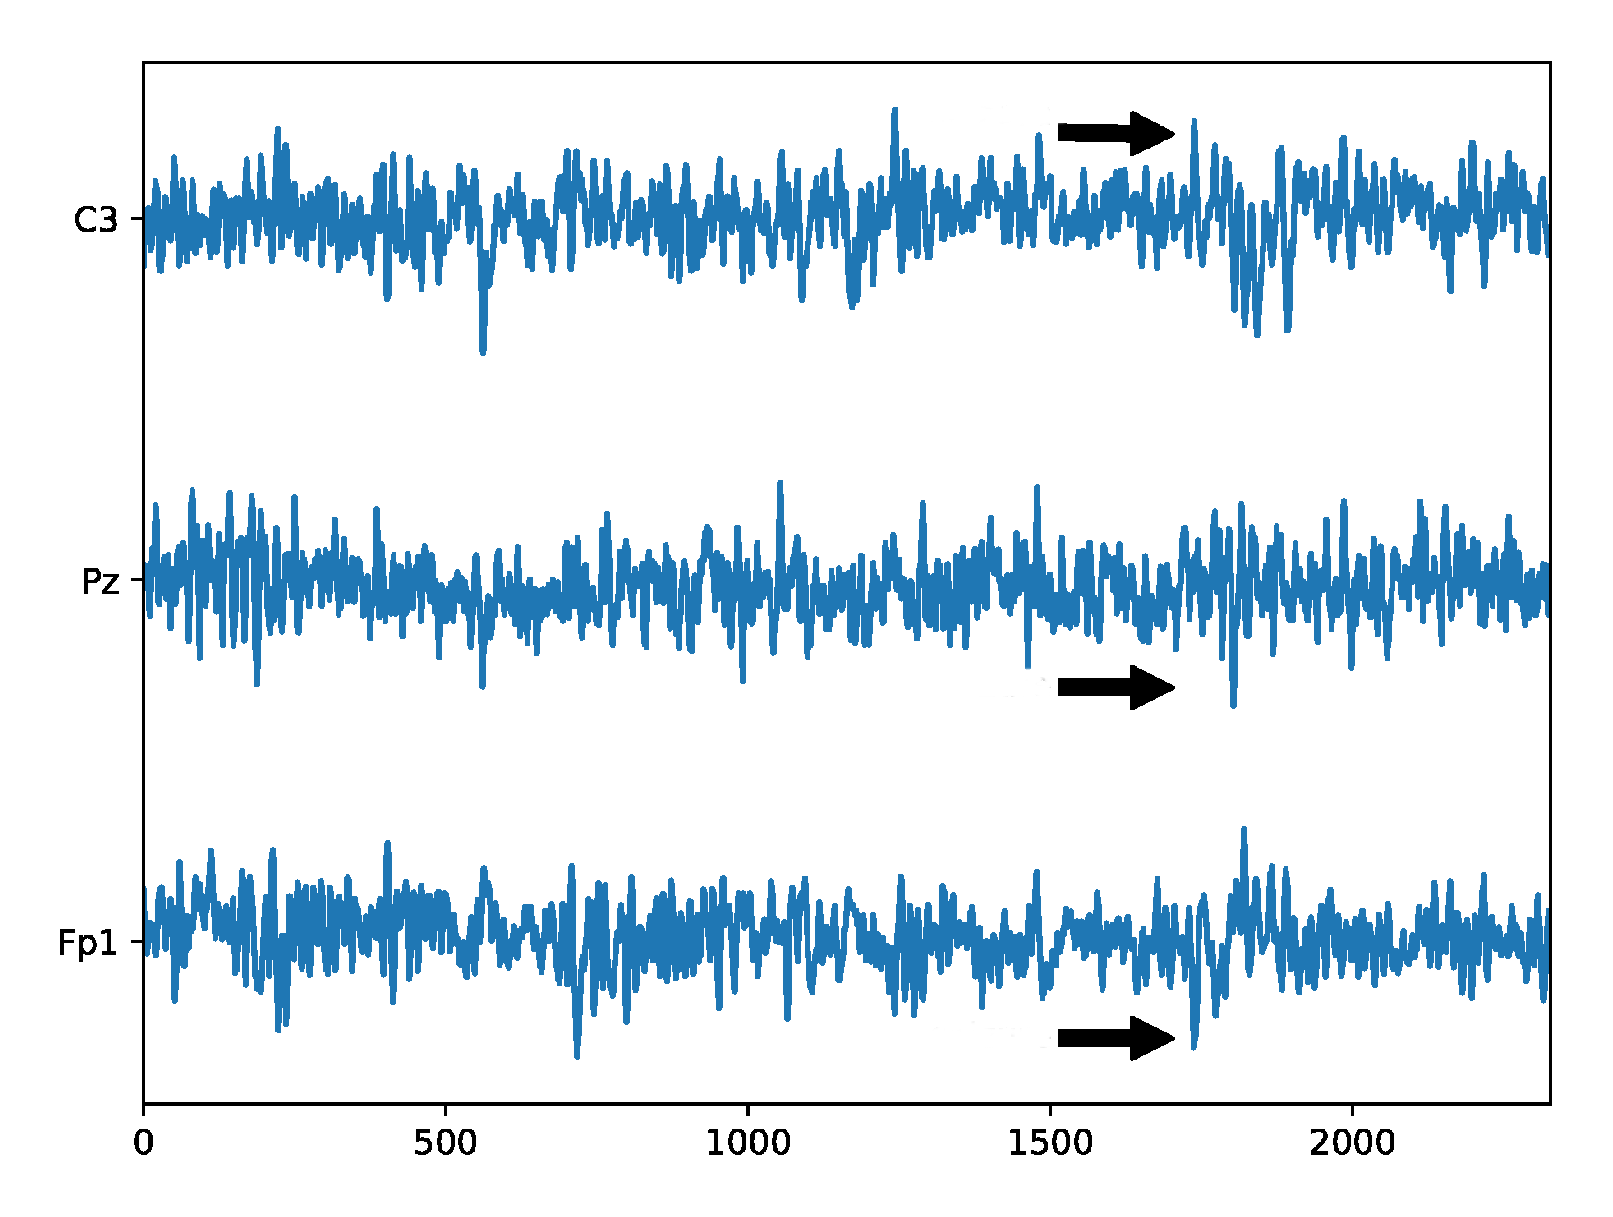
\includegraphics[scale=0.6]{IMG/mdpi/mouse_eeg.eps}
    \caption{Vybrané kanály myšího EEG na kterých je patrný epileptický záchvat. Data byly standartizovány. Začátek záchvatu je přibližně v $k\approx 1700$, což znázorňuje černá šipka.}
    \label{fig:eeg_seizure}
\end{figure}
\begin{figure}[ht!]
    \centering
    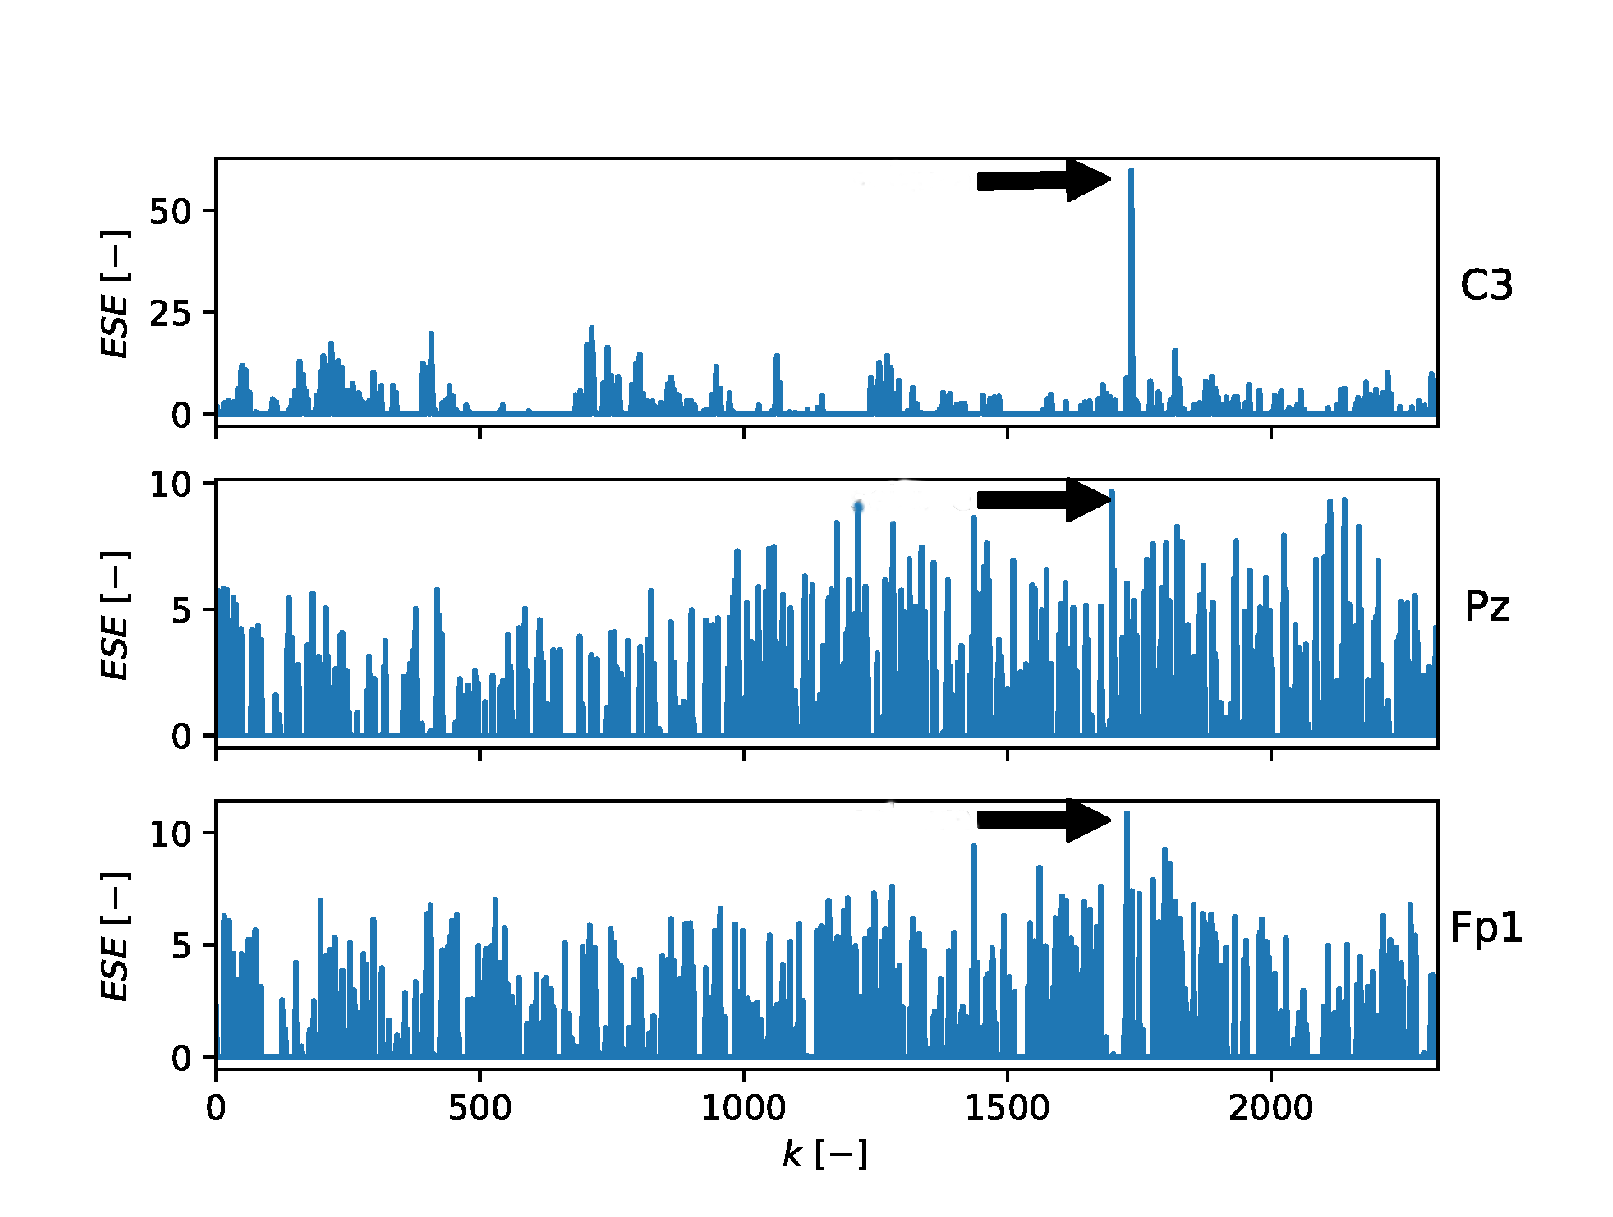
\includegraphics[scale=0.6]{IMG/mdpi/mouse_novelty.eps}
    \caption{Hodnota ESE pro vybrané kanály se záznamem myšího EEG ve kterých je patrný epileptický záchvat. V kanále C3 je v ESE výrazný nárůst po začátku záchvatu (přibližně v $k \approx 1700$), v porovnání s ostatními kanály. Černá šipka znázorňuje přibližný začátek epileptického záchvatu.}
    \label{fig:mouse_novelty}
\end{figure}


\subsection{Vyhodnocení úspěšnosti detekce skokové změny parametrů generátoru signálu}
Pro vyhodnocení úspěšnosti skokové změny parametrů generátoru signálu uvažujme generátor signálu s dvěma vstupy $x_1(k)$ a $x_2(k)$ a výstupem $y(k)$ ve tvaru
\begin{equation}
y(k)=a_1\cdot x_1(k)+a_2\cdot x_2(k)+a_3\cdot x_1(k) \cdot x_2(k)+v(k)
\end{equation}
kde člen $v(k)$ reprezentuje gaussovský aditivní šum s nulovou střední hodnotou a směrodatnou odchylkou $\sigma$. Počáteční hodnoty parametrů $a_1$, $a_2$ a $a_3$ jsou vygenerovány z rovnoměrného rozdělení $U(-1,1)$. V diskrétním časovém okamžiku $k=200$, dojde ke skokové změně těchto parametrů a jejich nová hodnota je opět náhodně vygenerována z rovnoměrného rozdělení $U(-1,1)$. Celkový počet vzorků experimentu je 400.
Použitý adaptivní filtr je stejný jako v předchozí případové studii detekce skokové změny parametrů generátoru signálu, viz kapitola \ref{chap:stepchange}. Parametry tohoto adaptivního filtru byly adaptovány algoritmem GNGD. Metoda POT byla zvolena podle rovnice \ref{eq:l1} a délka okna byla zvolena $n_s=1200$. Apriorní informace o parametrech GPD byla pro každý experiment získána pomoci 1200 vzorků, s počátečními hodnotami parametrů $a_1$, $a_2$ a $a_3$. Pro každý experiment byla vyhodnocena hodnota SNR jako
\begin{equation}\label{eq:snr}
SNR=10\log_{10}\frac{\sigma_s^2}{\sigma^2}
\end{equation}
kde $\sigma_s$  je hodnota směrodatné odchylky výstupu generátoru signálu během experimentu a $\sigma$ je směrodatná odchylka aditivního gaussovského šumu. Vyhodnocení přesnosti detekce bylo provedeno následujícím způsobem:
\begin{enumerate}
\item nastavení hodnoty směrodatné odchylky šumu $\sigma$
\item pro zvolenou hodnotu směrodatné odchylky $\sigma$ se provede 1000 experimentů, přičemž pro každý experiment jsou nově vygenerovány počáteční hodnoty parametrů generátoru signálu $a_1$, $a_2$ a $a_3$.
\item pro každý experiment je vyhodnocena úspěšnost detekce. Za úspěšnou detekci je považováno, pokud globální maximum ESE, ELBND, EL respektive chyby filtru je v mezích $k\geq 200$ a $k\leq 210$. 
\item vypočte se celková úspěšnost detekce pro danou hodnotu směrodatné odchylky (poměr počtu úspěšných detekcí k celkovému počtu experimentů)
\item pro každý experiment se vyhodnotí SNR podle \ref{eq:snr} a pak se pro zvolenou hodnotu $\sigma$ vypočítá průměrná hodnota $SNR$ pro všechny experimenty
\end{enumerate}
Vyhodnocení úspěšnosti detekce bylo vyhodnoceno pro dva případy. V prvním případě, byly hodnoty vstupů $x_1(k)$ a $x_2(k)$ generovány z rovnoměrného rozdělení $U(-1,1)$. Výsledky úspěšnosti detekce pro různé hodnoty směrodatných odchylek šumu $\sigma$ jsou zobrazeny na obrázku \ref{fig:step_uni_stats}. Výsledky jsou také shrnuty v tabulce XXX (viz příloha). Pro porovnání jsou zvoleny metody ELBND (výpočet podle rovnice \ref{eq:elbnd2}), LE s oknem $n_s=1200$ (výpočet podle rovnice \ref{eq:le_direct_padasip}) a velikost chyby adaptivního filtru $e$ (v grafu označeno jako ERR).

\begin{figure}[!ht]
    \centering
    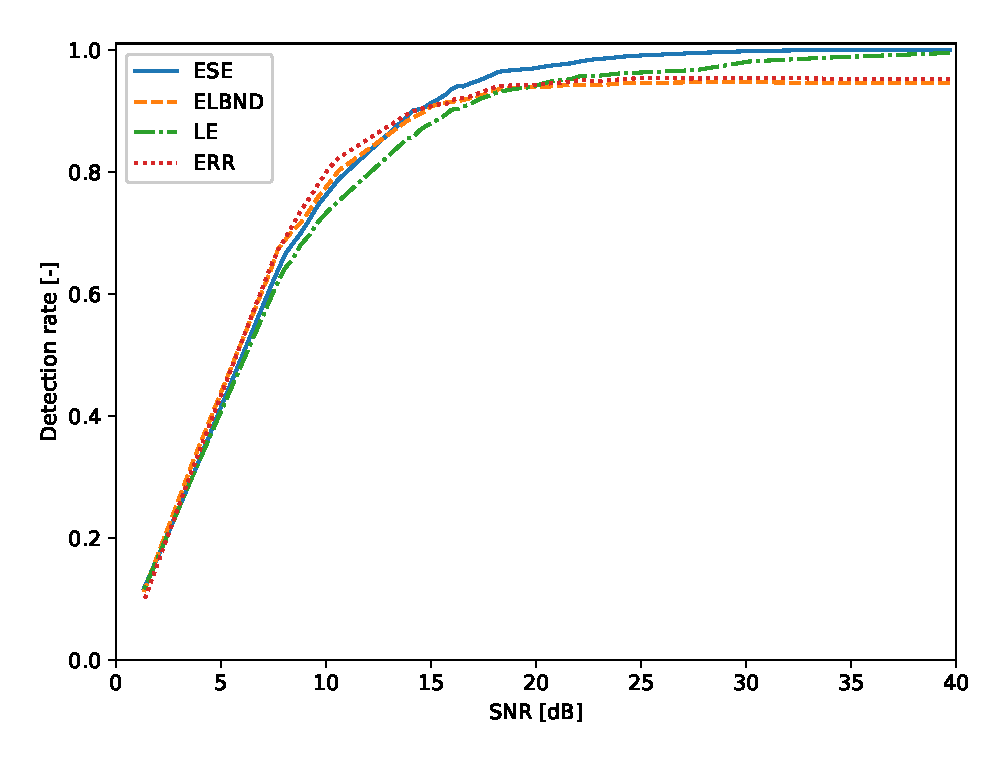
\includegraphics[scale=0.62]{IMG/mdpi/stepuni_stats.eps}
    \caption{Úspěšnost detekce skokové změny parametrů generátoru signálu. Hodnoty vstupů generátoru signálu jsou generovány z rovnoměrného rozdělení $U(-1,1)$. 
Pro hodnoty $SNR > 15$ $dB$ dosáhl algoritmus ESE vyšší úspěšnost než algoritmy  LE, ELBND a vyhodnocení pomocí chyby filtru (ERR). Pro $SNR > 33$ $dB$ dosáhl algoritmus ESE 100\% úspěšnost detekce.}
    \label{fig:step_uni_stats}
\end{figure}
Ve druhém případě byly hodnoty vstupů $x_1(k)$ a $x_2(k)$ generovány z normálního rozdělení. Vyhodnocení úspěšnosti detekce bylo provedeno stejně jako v případě popsaném výše. Výsledky ůspěšnosti detekce pro různé hodnoty směrodatných odchylek šumu $\sigma$ jsou zobrazeny na obrázku \ref{fig:step_norm_stats}. Uvedené výsledky v číselné podobě jsou uvedeny v tabulce XXX (viz příloha). Výpočet hodnot ELBND, LE a ERR bylo provedeno stejně jako ve výše uvedeném případě.

\begin{figure}[!h]
    \centering
    \includegraphics[scale=0.62]{IMG/mdpi/stepnorm_stats.eps}
    \caption{Úspěšnost detekce skokové změny parametrů signálu. Hodnoty vstupů generátoru signálu jsou generovány z normálního rozdělení $N(0,1)$. Pro hodnoty $SNR > 8$ $dB$ dosáhl algoritmus ESE  lepší úspěšnosti detekce než algoritmy LE, ELBND a vyhodnocení pomocí velikosti chyby predikce (ERR). Pro $SNR > 34$ $dB$ dosáhl algoritmus ESE 100\% úspěšnosti detekce.}
    \label{fig:step_norm_stats}
\end{figure}


\subsection{Vyhodnocení úspěšnosti detekce skokové změny trendu}
Pro vyhodnocení úspěšnosti změny trendu uvažujme výstup generátoru signálu $y(k)$ se dvěma vstupy $x_1(k)$ a $x_2(k)$ jehož výstup je definován jako
\begin{equation}\label{eq:trnd_stats}
    y(k) = x_1(k) + x_2(k) + 0.01 \cdot k + v(k)
\end{equation}
kde člen $v(k)$ reprezentuje aditivní gaussovký šum s nulovou střední hodnotou a směrodatnou odchylkou $\sigma$. V diskrétním časovém okamžiku $k=200$ se změní výstup generátoru signálu
\begin{equation}
    y(k) = x_1(k) + x_2(k) + (0.01 + a) \cdot k + v(k)
\end{equation}
přičemž parametr $a$ je vygenerován v každém experimentu z rovnoměrného rozdělení $U(-0.02,0.02)$. Počet vzorků experimentu je 400.
\par 
Struktura adaptivního filtru byla zvolena stejně jako v předcházející případové studii detekce změny trendu (viz kapitola \ref{chap:stepchange}). Adaptivní parametry filtru byly adaptovány algoritmem GNGD. Metoda POT pro algoritmus ESE byla zvolena jako \ref{eq:l1} a délka okna byla nastaven na $n_s=1200$. Apriorní informace o parametrech GPD byla získána na základě 1200 vzorků, ve kterých nedošlo ke změně trendu. 
\par 
Vyhodnocení přesnosti detekce změny trendu bylo provedeno následujícím způsobem:
\begin{enumerate}
\item nastavení hodnoty směrodatné odchylky šumu $\sigma$
\item pro zvolenou hodnotu směrodatné odchylky $\sigma$ se provede 1000 experimentů. V každém experimentu dojde v diskrétním časovém okamžiku $k=200$ k  novému vygenerování hodnoty parametru $a$ z rovnoměrného rozdělení $U(-0.02,0.02)$.
\item pro každý experiment je vyhodnocena úspěšnost detekce. Za úspěšnou detekci je považováno, pokud globální maximum ESE, ELBND, EL respektive chyby filtru je v mezích $k\geq 200$ a $k\leq 210$. 
\item vypočte se celková úspěšnost detekce pro danou hodnotu směrodatné odchylky (poměr počtu úspěšných detekcí k celkovému počtu experimentů)
\item pro každý experiment se vyhodnotí SNR podle \ref{eq:snr} a pak se pro zvolenou hodnotu $\sigma$ vypočítá průměrná hodnota $SNR$ pro všechny experimenty
\end{enumerate}

Vyhodnocení úspěšnosti detekce změny trendu bylo vyhodnoceno pro hodnoty vstupů $x_1(k)$ a $x_2(k)$ vygenerovány z rovnoměrného rozdělení $U(-1,1)$. Výsledky úspěšnosti detekce pro různé hodnoty směrodatných odchylek šumu $\sigma$ jsou zobrazeny na obrázku \ref{fig:trend_stats}. Výsledky jsou také shrnuty v tabulce XXX (viz příloha). Pro porovnání jsou zvoleny metody ELBND (výpočet podle rovnice \ref{eq:elbnd2}), LE s oknem $n_s=1200$ (výpočet podle rovnice \ref{eq:le_direct_padasip}) a velikost chyby adaptivního filtru $e$ (v grafu označeno jako ERR).

\begin{figure}[!ht]
    \centering
    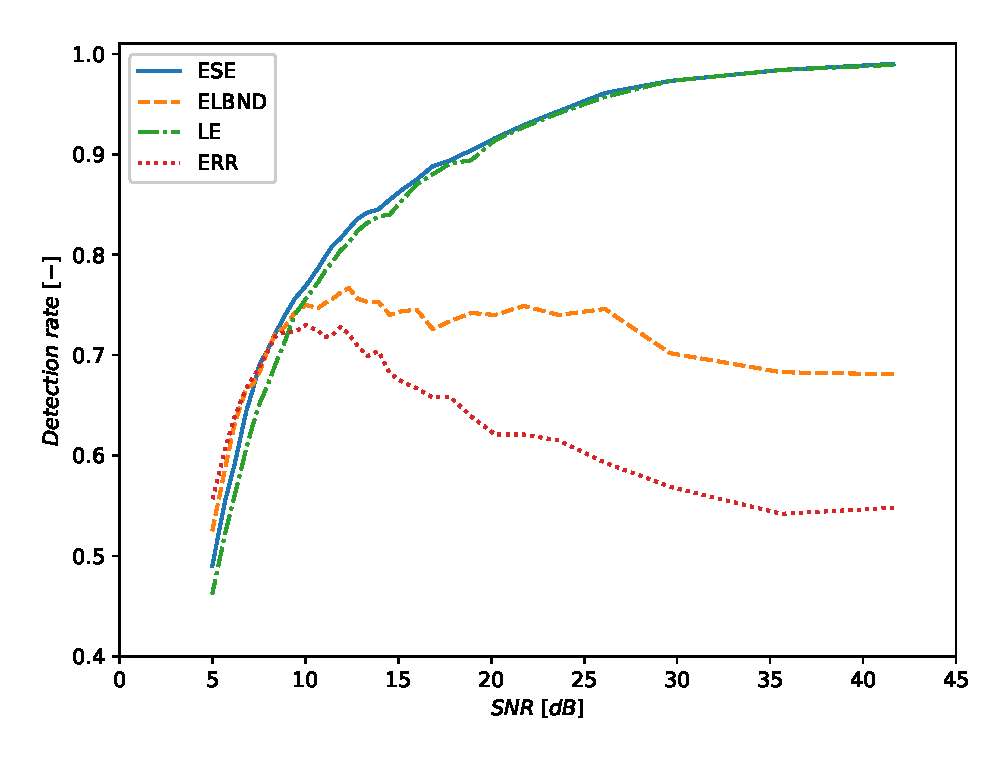
\includegraphics[scale=0.63]{IMG/mdpi/trendchange_stats.eps}
    \caption{Úspěšnost detekce změny trendu. Hodnoty vstupů generátoru signálu byly generovány z rovnoměrného rozdělení $U(-1,1)$. Pro hodnoty $SNR > 8$ $dB$ dosáhl algoritmus ESE větší úspěšnosti detekce než LE, ELBND a vyhodnocení pomocí velikosti chyby filtru.}
    \label{fig:trend_stats}
\end{figure}

\section{Vyhodnocení úspěšnosti detekce změny trendu a evaluace ROC křivky}
\#TODO
\section{Vyhodnocení výpočetní náročnosti metod odhadu parametrů zobecněného Paretova rozdělení}
Výsledky v této podkapitole byli publikovány v (můj shit). Cílem bylo určit výpočetní čas výpočtu parametrů GPD v typické aplikaci pro použití algoritmu ESE, který byl, v tomto případě, testován ne experimentu detekce skokové změny parametrů generátoru signálu.
\subsection{Motivace}
Detekce novosti v reálném čase je úloha, která nalézá své uplatnění nejen v oblasti detekci a diagnostiky v průmyslových aplikacích \cite{fault}, ale také např. v detekci narušení počítačových sítí \cite{data_streams} nebo v zabezpečovacích systémech \cite{surveilance}. Další oblastí uplatnění je např. mobilní robotika, která je specifická tím, že robot má k dispozici pouze limitovaný výpočetní výkon \cite{robotics_marslan,robotics}. Pro metody detekce novosti v reálném čase je tedy důležité, aby vynikali dostatečně nízkou výpočetní náročností. Z tohoto důvodu byli otestovány tři různé metody výpočtu parametrů GPD (viz kapitola \ref{chap:gpd}, protože tento výpočet je z hlediska použití algoritmu ESE potenciálně limitující z hlediska využitelnosti v aplikacích detekce v reálném čase. Jmenovitě byli otestovány tyto metody: metoda maximální věrohodnosti (ML), metoda momentů (MOM) a metoda kvazi-maximální věrohodnosti (QML) (více viz kapitola \ref{chap:gpd}). Výpočetní čas potřebný k určení parametrů GPD pomocí těchto metod byl vyhodnocen při experimentu, ve kterém dojde ke skokové změně parametrů generátoru signálu.
\subsection{Specifikace experimentu}
Vzhledem k povaze experimentu, který slouží k vyhodnocení výpočetní náročnosti různých metod určení parametrů GPD, a nikoliv k detekci novosti v nějakém komplexním procesu, byl zvolen jednoduchý lineární kombinační filtr (LNU), jehož výstup v diskrétním časovém okamžiku $k$ je definován jako
\begin{equation}\label{eq:gene_ese_1}
\hat{y}(k)=w_1\cdot x_1(k)+w_2\cdot x_2(k)+w_3\cdot x_3(k)
\end{equation}
a tento filtr je adaptován algoritmem NLMS (viz kapitola \ref{chap:nlms}), přičemž rychlost učení $\mu$ byla nastavena jako $\mu=0.8$.
\par 
Pro výstup generátoru signálu platí vztah
\begin{equation}
y(k)=x_1(k)+x_2(k)+x_3(k)+v(k)
\end{equation}
pro všechny $1 \leq k \leq 200$. Člen $v(k)$ reprezentuje aditivní gaussovský šum s nulovou střední hodnotou a směrodatnou odchylkou $\sigma_{noise}=0.1$. V diskrétním časovém okamžiku $k=201$ dojde ke změně generátoru signálu a jeho výstup přejde do tvaru
\begin{equation}
y(k)=0.7\cdot x_1(k)+1.2\cdot x_1(k)+1.1 \cdot x_1(k) + v(k)
\end{equation}
pro $201 \leq k \leq 400$. Hodnota všech vstupů generátoru signálu je v každém časovém okamžiku $k$ vybrána ze standartního rozdělení normálního rozdělení, takže $i$-tý vstup $x_i\sim \mathcal{N}(0,1)$. Změna parametrů signálu byla vybrána tak, aby nedošlo ke změně střední hodnoty signálu $y(k)$.
\par
Délka okna pro odhad parametrů GPD bylě během experimentu nastavena na $n_s=1200$. Metoda POT byla zvolena podle REF na 10\%. Před experimentem bylo pořízení 1200 vzorků vygenerovaných generátorem signálu definovaným vztahem \ref{eq:gene_ese_1}, na něž byla použita metoda POT, tak aby při experimentu v diskrétní časový okamžik $k=1$ byla hodnota ESE relevantní.
\par
Experiment byl proveden na PC s procesorem Intel(R) Core(TM) i5-7400 se 4mi jádry s taktovací frekvencí 3001 MHz a operační pamětí o velikosti 32 GB. Operační systém byl Windows 10 Pro, 64-bitová verze 10.0.18362. Kód byl napsán v Python 3.6.1 a byly použity knihovny Numpy 1.17.0 a Scipy 1.4.1.
Pro

\begin{figure}[h!]
	\label{fig:par_output}
	\centering
	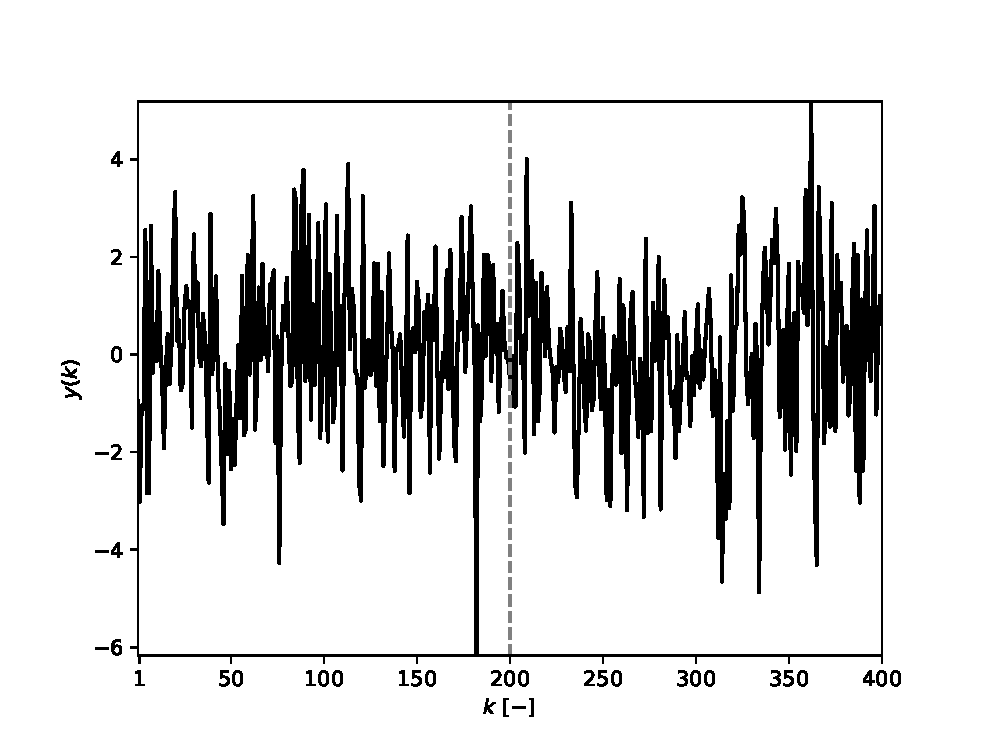
\includegraphics[scale=0.71]{IMG/appel_par/par_output.eps}
	\caption{Výstup adaptivního filtru během experimentu. Skoková změna parametrů generátoru signálu je zvýrazněná svislou vodorovnou čarou v diskrétním časovém okamžiku $k=200$.}
\end{figure}

\subsection{Výsledky a diskuze}


\begin{figure}[h!]
	\label{fig:par_ese}
	\centering
	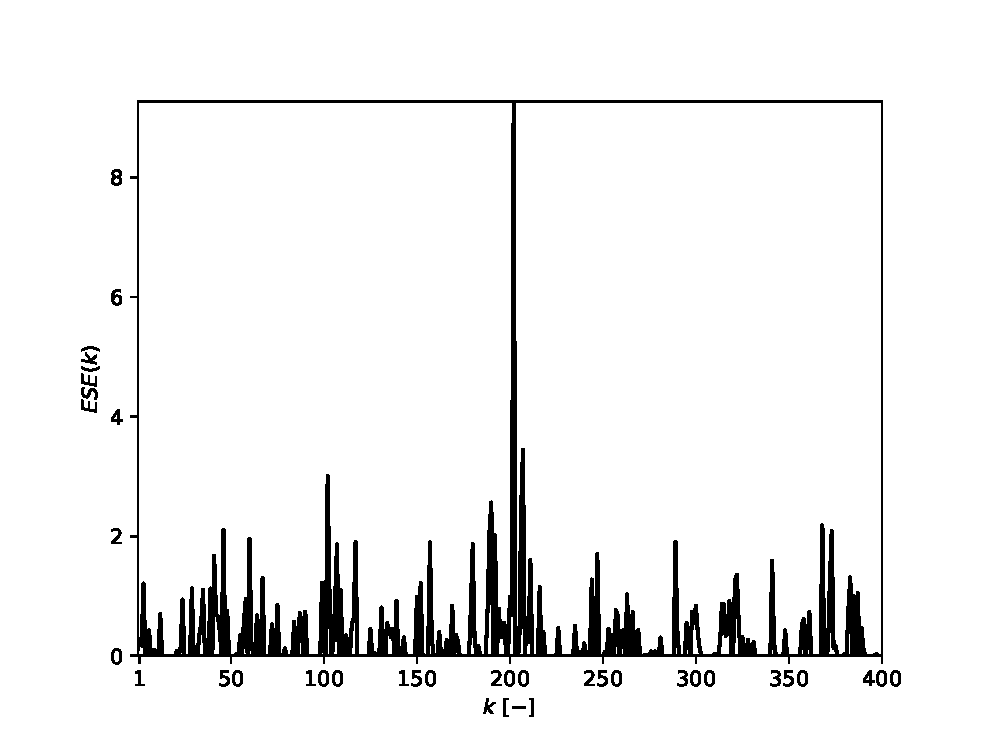
\includegraphics[scale=0.71]{IMG/appel_par/par_ese.eps}
	\caption{Hodnota ESE během experimentu. Globální maximum odpovídá změně parametrů generátoru signálu, resp. úspěšné detekci novosti.}
\end{figure}

\begin{figure}[h!]
	\label{fig:par_mu}
	\centering
	\includegraphics[scale=0.71]{IMG/appel_par/par_mu.eps}
	\caption{Hodnota parametru $\mu$ GPD pro všechny tři adaptivní váhy $w_1$, $w_2$, $w_3$ během experimentu detekce změn parametrů generátoru signálu. Svislá čára v diskrétním časovém okamžiku $k=200$ znázorňuje skokovou změnu parametrů generátoru signálu.}
\end{figure}

\begin{figure}[h!]
	\label{fig:par_gamma}
	\centering
	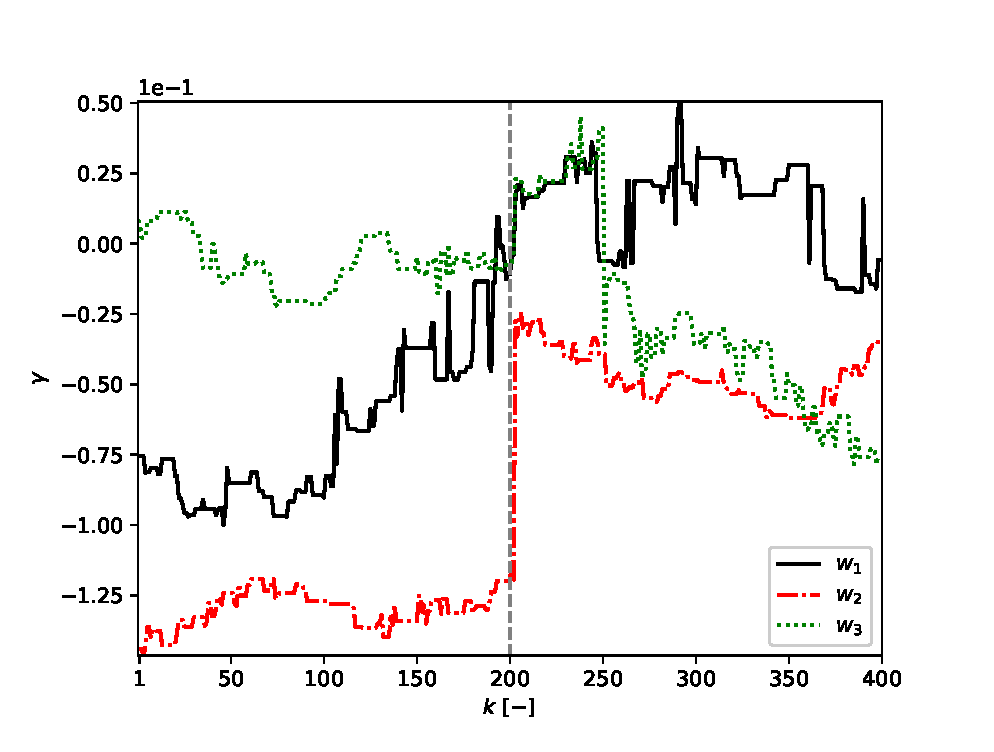
\includegraphics[scale=0.71]{IMG/appel_par/par_gamma.eps}
	\caption{Hodnota parametru $\gamma$ GPD pro všechny tři adaptivní váhy $w_1$, $w_2$, $w_3$ během experimentu detekce změn parametrů generátoru signálu. Svislá čára v diskrétním časovém okamžiku $k=200$ znázorňuje skokovou změnu parametrů generátoru signálu.}
\end{figure}

\begin{figure}[h!]
	\label{fig:par_sigma}
	\centering
	\includegraphics[scale=0.71]{IMG/appel_par/par_mu.eps}
	\caption{Hodnota parametru $\sigma$ GPD pro všechny tři adaptivní váhy $w_1$, $w_2$, $w_3$ během experimentu detekce změn parametrů generátoru signálu. Svislá čára v diskrétním časovém okamžiku $k=200$ znázorňuje skokovou změnu parametrů generátoru signálu.}
\end{figure}
Průměrný čas výpočtu $\overline{t}$ parametrů všech tří GPD (počet GPD odpovídá počtu adaptivních parametrů filtru) a odpovídající směrodatné odchylky $\sigma_t$ jsou uvedeny v následující tabulce \ref{tab:par_results}. Čas výpočtu je určený pro jeden experiment (400 vzorků).
\begin{table}[h!]

\centering
\caption{Tabulka průměrných časů výpočtu pro jednotlivé adaptivní váhy a odpovídajících směrodatných odchylek vybraných metod výpočtu parametrů GPD}
\begin{tabular}{|l|l||l|l|}
\hline
 & Metoda & $\overline{t}$ {[}ms{]} & $\sigma_t$ {[}ms{]} \\ \hline \hline
\multirow{3}{*}{$w_1$} & ML & $26.198$ & $3.396$ \\ \cline{2-4} 
 & QML & $0.354$ & $0.478$ \\ \cline{2-4} 
 & MOM & $\textbf{0.076}$ & $0.264$ \\ \hline
\multirow{3}{*}{$w_2$} & ML & $26.718$ & $2.302$ \\ \cline{2-4} 
 & QML & $0.337$ & $0.471$ \\ \cline{2-4} 
 & MOM & $\textbf{0.064}$ & $0.244$ \\ \hline
\multirow{3}{*}{$w_3$} & ML & $24.982$ & $1.964$ \\ \cline{2-4} 
 & QML & $0.395$ & $0.489$ \\ \cline{2-4} 
 & MOM & $\textbf{0.060}$ & $0.238$ \\ \hline

\end{tabular}
 \label{tab:par_results}
\end{table}

Z uvedených výsledků je patrné, že nejrychlejší metoda je MOM. Podstatnou nevýhodou této metody pro využití v aplikacích, které vyhodnocují data v reálném čase je její omezení na hodnoty parametrů GPD (viz kapitola \ref{chap:gpd}). Pokud parametry uvedené omezení nesplňují, vypočtené hodnoty nepřesné (resp. nesmyslné) a tedy nepoužitelné pro algoritmus ESE, který začne produkovat nepřesné výsledky. Z pohledu úlohy detekce novosti je diskutabilní, zda-li můžeme garantovat, že sledovaný proces po celou dobu bude splňovat uvedené omezení.
\par
Metoda, jejíž výpočetní čas byl nejvyšší je ML, což je vzhledem k iterativnímu určení parametrů GPD očekávatelné. Nevýhoda použití této metody tkví v  nemožnosti určit minimální resp. maximální počet iterací. Jednou z možností jak zrychlit nalezení parametrů je využití apriorní informace o hodnotách těchto parametrů. V rámci experimentu však byla využita pouze apriorní informace o parametru $\mu$, který odpovídá nejmenší hodnotě přírůstku vah, které byli získány metodou POT aplikovanou na plovoucí okno délky $n_s$.
\par
Dobrým kompromisem mezi výše uvedenými metodami je použití metody QML. Výpočetní čas této metody byl v uvedeném experimentu o dva řády kratší než ML a asi pětkrát delší než MOM. Pro každou z vyhodnocovaných vah byl kratší než $500$ $\mu s$.
\par 
Z provedeného experimentu je patrné, že použití algoritmu ESE pro aplikace v reálném čase je limitováno počtem parametrů filtru a rychlostí vzorkování monitorovaného procesu. 





\section{Případová studie použití algoritmu Learning Entropy a adaptivního fuzzy filtru pro detekci změn stavů bioprocesu} \label{chap:LE_fuzzy}
Cílem této studie je ověřit, že algoritmus LE, který byl doposud publikován s adaptivními filtry typu LNU a HONU, je možné použít i pro jiné typy adaptivních filtrů. Pro provedenou studii tak byl vybrán adaptivní fuzzy filtr (viz kapitola \ref{chap:fuzzyf}).
\subsection{Popis bioprocesu a specifikace problému}
Podle \cite{fermentace} je pro fermentační procesy, které probíhají v dávkovém režimu je podstatné, aby probíhalo správně dávkované živení substrátem. Pro tyto procesy je specifické, že se při nadměrných koncentracích stává substrát pro mikroorganismy toxickým a může dojít k tzv. přeživení a tím i zahubení těchto mikroorganismů. Naopak, v důsledku nedostatečného zábovení živinami může dojít k odumření kultivovaného organismu. Z tohoto pohledu se je tedy důležité v závislosti na koncentraci substrátu a stavu populace mikroorganismů měnit i strategii pro řízení procesu kultivace. Historicky byl stav bioprocesu klasifikován expertem, přičemž vyhodnocení bylo poměrně časově náročné a nebylo neobvyklé, že různí experti docházeli k rozdílným závěrům. Protože výnos fermentačního procesu je zásadním způsobem ovlivněn správnou klasifikací stavu ve kterém se právě nacházi, bylo by vhodné klasifikaci automatizovat a pokud možno zvýšit její přesnost. Tomuto problému je právě věnována publikace \cite{fermentace}, která řeší problém automatické klasifikace stavů bioprocesu kultivace bakterie \textit{Pseudomonas putida KT2442}. V této publikaci je navržen komplexní algoritmus pro online klasifikaci stavů bioprocesu. Autoři zde rozlišují celkem tři stavy bioprocesu kultivace \textit{Pseudomonas putida KT2442}, konkrétně:
\begin{enumerate}
    \item normální živení
    \item přeživení
    \item nedoživení
\end{enumerate}
Navržený algoritmus vyhodnocuje přísun vstupujících živin (Fm), respektive substrátu, a změny a trendu rozpuštěného kyslíku (DO), který je produkován bakteriemi \textit{Pseudomonas putida} a pomocí hřebenové regrese (v literatuře se vyskytuje také pod názvem Tichonova regularizace) je určován vývoj populace bakterií respektive stav bioprocesu. Vzhledem k tomu, že modely vývoje populace pro jednotlivé stavy jsou různé, mohlo by v průběhu experimentu dojít i k podstatným změnám v adaptivním modelu v okamžicích změn stavů kultivace. Tyto změny se mohli projevit neobvykle velkými přírůstky adaptivních parametrů. 
\par
Protože algoritmus Learning Entropy využívá přírůstku adaptivních parametrů, mohl by být vhodným nástrojem pro detekci změn stavů bioprocesu. Předpokládáme, že tedy existuje souvislost mezi změnami stavu bioprocesu a nárůstem Learning Entropy. Přestože může být proces kultivace bakterií \textit{Pseudonomas Putidas} modelován různými a různě složitými modely, pro využití algoritmu Learning Entropy se jeví výhodné použít jednoduché prediktory nebo sledovače. Dosud publikované články využívali pro algoritmus LE pouze FIR filtry, případně Volterrovy filtry, které mají adaptivní parametry v lineární závislosti. V tomto experimentu je použit adaptivní fuzzy filtr, jehož struktura je specifikována v kapitole \ref{chap:fuzzyf} a k jehož adaptaci byl použit algoritmus, který je uveden v kapitole \ref{chap:gd}.
\par
Použitý adaptivní fuzzy filtr má 9 pravidel ($M=9$), jehož $l$-té pravidlo je ve tvaru
\begin{equation}
    IF\;do(k-1)\; is\; A_1^l\;AND\;do(k-6)\;is\;A_2^l\;AND\;do(k-19)\;is\;A_3^l\;THEN\;do(k)\;is\;B^l
\end{equation}
kde $A_i^l$ je množina ve vstupním prostoru $U \subset R^3$ a $B^l$ je fuzzy množina ve výstupním prostoru $V \subset R$. V uvedeném pravidle jsou $do(k-1)$, $do(k-6)$, $do(k-19)$ a $do(k)$ lingvistické proměnné, které vyjadřují koncentraci rozpuštěného kyslíku $do$ v v diskrétních časových okamžicích $k$, $k-1$, $k-6$ respektive $k-19$, kde $k$ je diskrétní časový index. Vzhledem k tomu, že uvedený adaptivní fuzzy filtr používá Gaussovské funkce příslušnosti (viz kapitola \ref{chap:fuzzyf} je zobrazení popisující jeho výstup ve tvaru
\begin{equation}
    \hat{y}(\textbf{x}(k))=\frac{\sum_{j=1}^9 \overline{b}^j\Big[\prod_{i=1}^3 exp\Big(-\Big(\frac{x_i-\overline{x}_i^j}{\sigma_i^j}\Big)\Big)\Big]}{\sum_{j=1}^9 \Big[\prod_{i=1}^3 exp\Big(-\Big(\frac{x_i-\overline{x}_i^j}{\sigma_i^j}\Big)\Big)\Big]}
\end{equation}
kde vektor $\textbf{x}(k)$ je
\begin{equation}
    \textbf{x}(k)=[do(k-1),do(k-6),do(k-19)].
\end{equation}\
Protože hodnota koncetnrace rozpuštěného kyslíku je uváděna v procentech, platí pro všechna $x_i\in \langle 0;100\rangle$. K adaptování výše uvedeného filtru byl použit algoritmus gradient descent (viz kapitola \ref{chap:gd}. Maximální počet epoch byl stanoven na $q_{max}=100$ a požadovaná chyba predikce mezi výstupem adaptivního filtru a naměřenými daty na $\epsilon=0,001$. Rychlost učení byla během experimentů nastavena na $\mu=1$.
\par
Pro vyhodnocení novosti byla použita přímá verze algoritmu LE, takže
\begin{equation}\label{eq:le_putida}
    E(k)=max\{0, \sum_{j=1}^9 z(\abs{\Delta \overline{b^j})}-\beta\}
\end{equation}
kde funkce $z$ je dána rovnicí (XY) a $\beta$ je citlivostní parametr. Pro vyhodnocení novosti jsou tedy použity změny polohy středů množin ve výstupním prostoru, nikoliv změny parametrů fuzzy množin ve vstupním prostoru.

\subsection{Experiment a zhodnocení}
Experiment s použitím algoritmu LE a adaptivního fuzzy filtru byl uskutečněn na datech z kultivace bakterie \textit{Pseudonomas Putida}, který byl uskutečněn na Ústavu počítačové a řídicí techniky VŠCHT Praha. Celkem byly zpracovávány hodnoty ze dvou kultivací. Přestože bylo během experimentu měřena sada různých veličin (např. teplota, pH, atd.), osvědčil se pro použití LE signál rozpustěného kyslíku $do$ $[\%]$. Během experimentu bylo použito vzorkování $T=1$ $min$, což je vzhledem k rychlosti celého procesu dostatečně rychlé vzorkování. Počáteční nastavení parametrů adaptivního fuzzy filtru bylo provedeno tak, jak je popsáné v kapitole \ref{chap:gd}. Podstatný vliv na výsledek detekce změn stavu bioprocesu měla volba volba délky okna pro vyhodnocení změn adaptabilních parametrů filtru $M_{ND}$. Na základě experimentů s různými délkami byla nakonec zvolena délka okna $M_{ND}=20$.
\par
Na následujících obrázcích je znázorněn průběh signálu $do$ během první kultivace (viz obrázek \ref{fig:artep_1}), chyba predikce (viz obrázek \ref{fig:artep_3}) a odpovídající hodnoty $LE$ společně se stavy bioprocesu (viz obrázek \ref{fig:artep_4}). Význam stavů bioprocesu znázorněných na obrázku \ref{fig:artep_3} respektive obrázku \ref{fig:artep_6} jsou: 1 - nedoživení, 2 - živení, 3 - přeživení. Aby byli detekovány všechny změny stavu bioprocesů, byla stanovena hodnota parametru $\beta=2,58$ (viz rovnice \ref{eq:le_putida}).
\par
Data z druhé kultivace byla použita k ověření správného nastavení parametru $\beta$.  Obrázek \ref{fig:artep_2} zobrazuje průběh signálu $do$ během druhého experimentu. Chyba predikce adaptivního fuzzy filtru je zobrazena na obrázku \ref{fig:artep_5}.  Obrázek \ref{fig:artep_6} zobrazuje stavy bioprocesu během kultivace a odpovídající hodnoty $LE$. S tímto nastavením parametru $\beta$ se podařilo detekovat pouze tři změny bioprocesu. Nicméně pro jiné hodnoty délky okna $M_{ND}$ a hodnoty parametru $\beta$ se tyto změny detekovat podařilo. Je tedy zřejmé, že pro praktické použití je správná volba obou parametrů zásadní. Vzhledem k malému množství dat a časové náročnosti kultivace nebylo možné použít nějakou validační metodu. 

\begin{figure}
    \centering
    \includegraphics[scale=0.8]{IMG/artep/artep17_1.png}
    \caption{Průběh signálu $do$ během první kultivace}
    \label{fig:artep_1}
\end{figure}

\begin{figure}
    \centering
    \includegraphics[scale=0.8]{IMG/artep/artep17_3.png}
    \caption{Chyba predikce $e$ během první kultivace}
    \label{fig:artep_3}
\end{figure}

\begin{figure}
    \centering
    \includegraphics[scale=0.8]{IMG/artep/artep17_4.png}
    \caption{Stav bioprocesu a hodnota $LE$ první kultivace}
    \label{fig:artep_5}
\end{figure}

\begin{figure}
    \centering
    \includegraphics[scale=0.8]{IMG/artep/artep17_2.png}
    \caption{Průběh signálu $do$ během druhé kultivace}
    \label{fig:artep_2}
\end{figure}

\begin{figure}
    \centering
    \includegraphics[scale=0.8]{IMG/artep/artep17_5.png}
    \caption{Chyba predikce $e$ během druhé kultivace}
    \label{fig:artep_4}
\end{figure}

\begin{figure}
    \centering
    \includegraphics[scale=0.8]{IMG/artep/artep17_6.png}
    \caption{Stav bioprocesu a hodnota $LE$ během druhé kultivace}
    \label{fig:artep_6}
\end{figure}




 
\chapter{Závěr}
Předložená dizertační práce je věnována použití adaptivních systémů při analýze dat. Z chronologického pohledu je prvním výstupem během zpracování této práce případová studie algoritmu Learning Entropy pro detekci změn stavu bioprocesu s využitím adaptivního fuzzy filtru \cite{artep}, více viz příloha \ref{chap:LE_fuzzy}. Dále byla úspěšně vyzkoušena detekce fázové změny v krystalografických datech pomocí adaptivního filtru a zobecněného rozdělení extrémních hodnot \cite{asr}. Zobecněné rozdělení extrémních hodnot bylo také využito v případové studii skokové změny parametrů generátoru signálu \cite{appel1}. 
\par 
Za zásadní výsledek lze považovat nový originální algoritmus pro detekci novosti, který vyhodnocuje přírůstky adaptivních vah filtru, Extreme Seeking Entropy \cite{ese_mdpi} (viz kapitola \ref{chap:ese}). Tento algoritmus byl otestován v následujících případových studiích (viz kapitola \ref{chap:vysledky}): detekce pertubace v chaotické časové řadě získané řešením Mackey-Glassovy rovnice, detekce změny rozptylu šumu v náhodném datovém toku, detekce skokové změny parametrů generátoru signálu, detekce náhlé absence šumu, detekce změny trendu a při detekci epilepsie v myším EEG. Pro detekci skokové změny trendu a skokové změny parametrů signálu byla vyhodnocena úspěšnost této detekce a výsledky porovnány s výsledky algoritmů Learning Entropy a Error and Learning Based Novelty Detection, přičemž v obou případech byla úspěšnost detekce algoritmu ESE vyšší pro téměř všechny vyhodnocované hodnoty SNR. Pro hodnotu $SNR>34$ $dB$ dosáhl algoritmus při detekci skokové změny parametrů generátoru signálu $100\%$ úspěšnost. Při detekci změny trendu měl algoritmus ESE pro hodnoty $SNR>8$ $dB$ větší úspěšnost detekce než srovnávané algoritmy LE a ELBND. Výše uvedené výsledky byly publikovány v \cite{ese_mdpi}.
\par Pro možné použití v aplikacích detekce v reálném čase byla experimentálně zjišťována výpočetní časová náročnost různých metod odhadů parametrů zobecněného Paretova rozdělení v případě použití algoritmu ESE při detekci skokové změny parametrů \cite{appel2}. Výsledkem je porovnání 3 různých metod odhadu parametrů. Limitujícím faktorem použití ESE v reálném čase je v zásadě počet adaptivních parametrů filtru, které je potřeba vyhodnocovat a samozřejmě rychlost vzorkování monitorovaného signálu.
\par Pro odhad úspěšnosti detekce novosti pomocí algoritmu ESE byla také vyhodnocena ROC křivka v případě detekce změny trendu signálu s různými poměry SNR a byly určeny příslušné plochy pod těmito ROC křivkami \cite{appel3}. Dosažené výsledky byly opět porovnány s algoritmy LE a ELBND a bylo ověřeno, že pro hodnoty $SNR \leq 30$ $dB$ dosahuje algoritmus ESE lepších výsledků. Pro vyšší hodnoty $SNR$ pak byly výsledky ESE srovnatelné s výsledky LE.  Cílem této studie bylo zjistit jak dobře dokáže algoritmus ESE separovat nová data v závislosti na volbě prahu, který rozhoduje o tom zda data obsahují novost či nikoliv. Pro představu ještě uveďme, že např. pro hodnotu $SNR=16.2$ $dB$ bylo dosaženo úspěšnosti detekce $90.42\%$.
\par
Stanovené cíle dizertační práce (viz \ref{chap:cile}) tak lze, na základě výše uvedených výsledků, považovat za splněné.

\section{Možné směry budoucího výzkumu}
V budoucnu se nabízí rozvíjet téma využití adaptivních systémů ve zpracování dat několika směry. Potenciální využití vyhodnocení změn vah adaptivních systémů lze využít v optimalizaci velikosti datasetů v oblasti hlubokého učení, což by mohlo výrazně snížit časovou náročnost učení hlubokých sítí. Za účelem snížení výpočetního času algoritmu ESE je potřeba vyzkoušet další metody odhadu parametrů zobecněného Paretova rozdělení a vyzkoušet adaptivní metody volby velikosti prahu pro metodu Peak-over-threshold. Zajímavým tématem je také vliv šumu a jeho typu na velikost přírůstků adaptivních vah filtrů a jejich pravděpodobnostní rozdělení. V neposlední řadě se nabízí otázka, jak ovlivní typ kriteriální funkce pro optimalizaci adaptivního filtru výsledky algoritmu ESE a je-li možné různé kriteriální funkce využívat k detekci novosti, případně pomocí nich typ novosti klasifikovat. 


\renewcommand{\bibname}{Publikace autora}
\begin{thebibliography}{A}
\bibitem{ese_mdpi}VRBA, Jan; MAREŠ, Jan. Introduction to Extreme Seeking Entropy. Entropy, 2020, 22.1: 93.
\bibitem{ijcnn}BUKOVSKÝ, Ivo, CEJNEK, Matouš, VRBA, Jan, HOMMA, Noryasu. Study of Learning Entropy for Onset Detection of Epileptic Seizures in EEG Time Series. \textit{The 2016 International Joint Conference on Neural Networks (IJCNN 2016)}. IEEE WCCI 2016, Vancouver, 2016. ISBN 978-1-5090-0620-5
\bibitem{appel1}VRBA, Jan. Adaptive Novelty Detection with Generalized Extreme Value Distribution. In: 2018 International Conference on Applied Electronics (AE). IEEE, 2018. p. 1-4.
\bibitem{cyril}OSWALD, Cyril, CEJNEK, Matouš, VRBA, Jan, BUKOVSKÝ, Ivo. Novelty Detection in System Monitoring and Control with HONU. In: ZHANG, Ming. \textit{ Aplied artificial higher order neural networks for control and recognition}. Hershey, PA: Information Science Reference, an imprint of IGI Global, 2016. ISBN 9781522500643.
\bibitem{roboti}VRBA, Jan, et al. An Automated Platform for Microrobot Manipulation. In: International Workshop on Soft Computing Models in Industrial and Environmental Applications. Springer, Cham, 2020. p. 255-265.
\bibitem{bila1}BÍLA, Jiří; VRBA, Jan. The Detection and Interpretation of Emergent Situations in ECG Signals. In: International Conference on Soft Computing-MENDEL. Springer, Cham, 2016. p. 264-275.
\bibitem{ijcnn3}MOJZES, Matej, et al. Feature selection via competitive levy flights. In: 2016 International Joint Conference on Neural Networks (IJCNN). IEEE, 2016. p. 3731-3736.
\bibitem{bila2}BILA, Jiri; NOVAK, Martin; VRBA, Jan. Detection of emergent situations in complex systems represented by algebras of transformations. In: MATEC Web of Conferences. EDP Sciences, 2016. p. 02035.
\bibitem{artep}VRBA, Jan. Využití fuzzy systémů a algoritmu learning entropy pro detekci změn stavů bioprocesu. In: \textit{Automatizacia a riadenie v teorii a praxi ARTEP 2017}. 11. ročník konferencie odbornikov z univerzit, vysokých škol a praxe. Technická univerzita Košice, 2017. ISBN 978-80-553-3075-4.
\bibitem{asr}VRBA, Jan, ŠKOLÁKOVÁ, Andrea. Adaptivní metoda detekce novosti, XLIII. In: \textit{ Seminář ASŘ 2018}. VŠB TU Ostrava, 2018.
\bibitem{artep2}BUKOVSKÝ, Ivo, OSWALD, Cyril, VRBA, Jan. Případová studie použití entropie učení pro adaptivní detekci při řízení spalování tuhých paliv. In: \textit{Automatizácia a riadenie v teórii a praxi 2015}. Technická univerzita Košice, 2015. ISBN 978-80-553-1968-1.
\bibitem{appel2}VRBA, Jan; MAREŠ, Jan. Computational Performance of the Parameters Estimation in Extreme Seeking Entropy Algorithm. In: 2020 International Conference on Applied Electronics (AE). IEEE, 2020. p. 1-4.
\bibitem{appel3}VRBA, Jan; MAREŠ, Jan. ROC Analysis of Extreme Seeking Entropy for Trend Change Detection. In: 2020 International Conference on Applied Electronics (AE). IEEE, 2020. p. 1-4.
\end{thebibliography}


\renewcommand{\bibname}{Literatura}
\begin{thebibliography}{L}

\bibitem{fermentace}MAREŠ, Jan, et al. Process state classification of fed-batch fermentation based on process variables analysis. Biochemical Engineering Journal, 2016, 112: 178-185.
\bibitem{rls_mit}ROWELL, D. 2.161 Signal Processing: Continuous and Discrete, Fall 2008. 2008.
\bibitem{rls_kalman}MANDIC, Danilo P.; KANNA, Sithan; CONSTANTINIDES, Anthony G. On the intrinsic relationship between the least mean square and Kalman filters [Lecture Notes]. IEEE Signal Processing Magazine, 2015, 32.6: 117-122.
\bibitem{proakis}PROAKIS, John G. a Dimitris G. MANOLAKIS. Digital signal processing: principles, algorithms, and applications. 3rd ed. Upper Saddle River, N.J.: Prentice Hall, 1996. ISBN 0133737624.
\bibitem{eeg}OOSTENVELD, Robert; PRAAMSTRA, Peter. The five percent electrode system for high-resolution EEG and ERP measurements. Clinical neurophysiology, 2001, 112.4: 713-719.
\bibitem{haykin}HAYKIN, Simon S. Adaptive filter theory. Fifth edition. vyd. Upper Saddle River, New Jersey: Pearson, 2014. ISBN 978-0-13-267145-3.
\bibitem{dirac}STRICHARTZ, Robert S. A guide to distribution theory and Fourier transforms. World Scientific Publishing Company, 2003.
\bibitem{kvantizace}GERSHO, Allen; GRAY, Robert M. Vector quantization and signal compression. Springer Science \& Business Media, 2012.
\bibitem{ivoLE2}BUKOVSKY, Ivo; KINSNER, Witold; HOMMA, Noriyasu. Learning Entropy as a Learning-Based Information Concept. Entropy, 2019, 21.2: 166.
\bibitem{ivoLE1}BUKOVSKY, Ivo. Learning entropy: Multiscale measure for incremental learning. Entropy, 2013, 15.10: 4159-4187.
\bibitem{elbnd1}CEJNEK, Matous; BUKOVSKY, Ivo. Concept drift robust adaptive novelty detection for data streams. Neurocomputing, 2018, 309: 46-53.
\bibitem{elbnd2} CEJNEK, Matous; BUKOVSKY, Ivo. Influence of type and level of noise on the performance of an adaptive novelty detector. In: 2017 IEEE 16th International Conference on Cognitive Informatics \& Cognitive Computing (ICCI* CC). IEEE, 2017. p. 373-377.
\bibitem{elbnd3}CEJNEK, Matous; BUKOVSKY, Ivo; VYSATA, Oldrich. Adaptive classification of EEG for dementia diagnosis. In: 2015 International Workshop on Computational Intelligence for Multimedia Understanding (IWCIM). IEEE, 2015. p. 1-5.
\bibitem{fault}GERTLER, Janos. Fault detection and diagnosis in engineering systems. CRC press, 1998.
\bibitem{data_streams}YU, Kangqing, et al. Real-time Outlier Detection over Streaming Data. In: 2019 IEEE SmartWorld, Ubiquitous Intelligence \& Computing, Advanced \& Trusted Computing, Scalable Computing \& Communications, Cloud \& Big Data Computing, Internet of People and Smart City Innovation (SmartWorld/SCALCOM/UIC/ATC/CBDCom/IOP/SCI). IEEE, 2019. p. 125-132.
\bibitem{surveilance}
RAMEZANI, Ramin; ANGELOV, Plamen; ZHOU, Xiaowei. A fast approach to novelty detection in video streams using recursive density estimation. In: 2008 4th International IEEE Conference Intelligent Systems. IEEE, 2008. p. 14-2-14-7.
\bibitem{robotics_marslan}
MARSLAND, Stephen; NEHMZOW, Ulrich; SHAPIRO, Jonathan. On-line novelty detection for autonomous mobile robots. Robotics and Autonomous Systems, 2005, 51.2-3: 191-206.
\bibitem{robotics}
NEHMZOW, Ulrich, et al. Novelty detection as an intrinsic motivation for cumulative learning robots. In: Intrinsically Motivated Learning in Natural and Artificial Systems. Springer, Berlin, Heidelberg, 2013. p. 185-207.
\bibitem{scarrot2012review}SCARROTT, Carl; MACDONALD, Anna. A review of extreme value threshold es-timation and uncertainty quantification. REVSTAT–Statistical Journal, 2012, 10.1: 33-60.
\bibitem{mackey}MACKEY, Michael C.; GLASS, Leon. Oscillation and chaos in physiological control systems. Science, 1977, 197.4300: 287-289.
\bibitem{dead}SPANGENBERG, Mariana, et al. Detection of variance changes and mean value jumps in measurement noise for multipath mitigation in urban navigation. Navigation, 2010, 57.1: 35-52.
\bibitem{diagnosis}MAURYA, Mano Ram; RENGASWAMY, Raghunathan; VENKATASUBRAMANIAN, Venkat. Fault diagnosis using dynamic trend analysis: A review and recent developments. Engineering Applications of artificial intelligence, 2007, 20.2: 133-146.
\bibitem{stepchange}L'ECUYER, Pierre. History of uniform random number generation. In: 2017 Winter Simulation Conference (WSC). IEEE, 2017. p. 202-230.
\bibitem{roc_orig}EGAN, J.P. Signal Detection Theory and ROC-analysis. Academic Press, 1975. Academic Press series in cognition and perception. ISBN 978-0-12-232850-3. 
\bibitem{roc_bible}FAWCETT, Tom. An introduction to ROC analysis. Pattern recognition letters, 2006, 27.8: 861-874.

\bibitem{mom_orig}HOSKING, Jonathan RM; WALLIS, James R. Parameter and quantile estimation for the generalized Pareto distribution. Technometrics, 1987, 29.3: 339-349.
\bibitem{DuMouchel}DUMOUCHEL, William H. Estimating the stable index $\alpha$ in order to measure tail thickness: a critique. the Annals of Statistics, 1983, 1019-1031.
\bibitem{history}HALD, Anders. A History of Mathematical Statistics from 1750 to 1930. New York: Wiley, 1998.
\bibitem{stat_bible}MONTGOMERY, Douglas C.; RUNGER, George C. Applied Statistics and Probability for Engineers. 2007.
\bibitem{grim}GRIMSHAW, Scott D. Computing maximum likelihood estimates for the generalized Pareto distribution. Technometrics, 1993, 35.2: 185-191.
\bibitem{SmithML}SMITH, Richard L. Maximum likelihood estimation in a class of nonregular cases. Biometrika, 1985, 72.1: 67-90.
\bibitem{Luceno}LUCENO, Alberto. Fitting the generalized Pareto distribution to data using maximum goodness-of-fit estimators. Computational Statistics \& Data Analysis [online]. 2006, 51(2), 904-917 [cit. 2020-09-25]. ISSN 01679473. Dostupné z: doi:10.1016/j.csda.2005.09.011
\bibitem{zhang1}ZHANG, Jin. Likelihood moment estimation for the generalized Pareto distribution. Australian \& New Zealand Journal of Statistics, 2007, 49.1: 69-77.
\bibitem{zhao}ZHAO, Xu, et al. A New Parameter Estimator for the Generalized Pareto Distribution under the Peaks over Threshold Framework. Mathematics, 2019, 7.5: 406.
\bibitem{park}PARK, Myung Hyun; KIM, Joseph HT. Estimating extreme tail risk measures with generalized Pareto distribution. Computational Statistics \& Data Analysis, 2016, 98: 91-104.
\bibitem{gpd_est}DE ZEA BERMUDEZ, P.; KOTZ, Samuel. Parameter estimation of the generalized Pareto distribution—Part I. Journal of Statistical Planning and Inference, 2010, 140.6: 1353-1373.
\bibitem{miljkovic}MILJKOVIĆ, Dubravko. Review of novelty detection methods. In: The 33rd International Convention MIPRO. IEEE, 2010. p. 593-598.
\bibitem{zimek}ZIMEK, Arthur; FILZMOSER, Peter. There and back again: Outlier detection between statistical reasoning and data mining algorithms. Wiley Interdisciplinary Reviews: Data Mining and Knowledge Discovery, 2018, 8.6: e1280.
\bibitem{markou1}MARKOU, Markos; SINGH, Sameer. Novelty detection: a review—part 1: statistical approaches. Signal processing, 2003, 83.12: 2481-2497.
\bibitem{markou2}MARKOU, Markos; SINGH, Sameer. Novelty detection: a review—part 2:: neural network based approaches. Signal processing, 2003, 83.12: 2499-2521.
\bibitem{pimentel}PIMENTEL, Marco AF, et al. A review of novelty detection. Signal Processing, 2014, 99: 215-249.
\bibitem{set_member}GOLLAMUDI, Sridhar, et al. Set-membership filtering and a set-membership normalized LMS algorithm with an adaptive step size. IEEE Signal Processing Letters, 1998, 5.5: 111-114.
\bibitem{diniz1}DINIZ, Paulo SR; YAZDANPANAH, Hamed. Data censoring with set-membership algorithms. In: 2017 IEEE Global Conference on Signal and Information Processing (GlobalSIP). IEEE, 2017. p. 121-125.
\bibitem{set_member_robot}ZHOU, Bo, et al. Multi-sensor fusion robust localization for indoor mobile robots based on a set-membership estimator. In: 2015 IEEE International Conference on Cyber Technology in Automation, Control, and Intelligent Systems (CYBER). IEEE, 2015. p. 157-162.
\bibitem{set_member_robot_voda}JAULIN, Luc. Robust set-membership state estimation; application to underwater robotics. Automatica, 2009, 45.1: 202-206.
\bibitem{set_member_robot_chyba}HUANG, Jian; WANG, Yuan; FUKUDA, Toshio. Set-membership-based fault detection and isolation for robotic assembly of electrical connectors. IEEE Transactions on Automation Science and Engineering, 2016, 15.1: 160-171.
\bibitem{diniz0}DINIZ, Paulo Sergio Ramirez. Adaptive filtering: algorithms and practical implementation. 3rd ed. New York: Springer, 2008. ISBN 978-0-387-31274-3.
\bibitem{auto1}NICOLAU, Miguel, et al. A hybrid autoencoder and density estimation model for anomaly detection. In: International Conference on Parallel Problem Solving from Nature. Springer, Cham, 2016. p. 717-726.
\bibitem{auto2}AN, Jinwon; CHO, Sungzoon. Variational autoencoder based anomaly detection using reconstruction probability. Special Lecture on IE, 2015, 2.1: 1-18.
\bibitem{auto3}MARCHI, Erik, Fabio VESPERINI, Florian EYBEN, Stefano SQUARTINI a Bjorn SCHULLER. A novel approach for automatic acoustic novelty detection using a denoising autoencoder with bidirectional LSTM neural networks. In: 2015 IEEE International Conference on Acoustics, Speech and Signal Processing (ICASSP) [online]. IEEE, 2015, 2015, s. 1996-2000 [cit. 2020-09-03]. ISBN 978-1-4673-6997-8. Dostupné z: doi:10.1109/ICASSP.2015.7178320
\bibitem{auto4}FENG, Qingsong, et al. Anomaly detection of spectrum in wireless communication via deep auto-encoders. The Journal of Supercomputing, 2017, 73.7: 3161-3178.
\bibitem{auto5}DOMINGUES, Rémi, et al. Deep Gaussian Process autoencoders for novelty detection. Machine Learning, 2018, 107.8-10: 1363-1383.
\bibitem{auto6}BHATTACHARJEE, Supritam; MANDAL, Devraj; BISWAS, Soma. Autoencoder based novelty detection for generalized zero shot learning. In: 2019 IEEE International Conference on Image Processing (ICIP). IEEE, 2019. p. 3646-3650.
\bibitem{auto7}KIEU, Tung, et al. Outlier Detection for Time Series with Recurrent Autoencoder Ensembles. In: IJCAI. 2019. p. 2725-2732.
\bibitem{auto8}MARCHI, Erik, et al. Deep recurrent neural network-based autoencoders for acoustic novelty detection. Computational intelligence and neuroscience, 2017, 2017.
\bibitem{auto9}KAWACHI, Yuta; KOIZUMI, Yuma; HARADA, Noboru. Complementary set variational autoencoder for supervised anomaly detection. In: 2018 IEEE International Conference on Acoustics, Speech and Signal Processing (ICASSP). IEEE, 2018. p. 2366-2370.
\bibitem{auto10}WANG, Xuhong, et al. adVAE: A self-adversarial variational autoencoder with Gaussian anomaly prior knowledge for anomaly detection. Knowledge-Based Systems, 2020, 190: 105187.
\bibitem{gmm1}REYNOLDS, Douglas A. Gaussian Mixture Models. Encyclopedia of biometrics, 2009, 741.
\bibitem{gmm2}HEYNS, Theo; HEYNS, Philippus Stephanus; DE VILLIERS, Johan Pieter. Combining synchronous averaging with a Gaussian mixture model novelty detection scheme for vibration-based condition monitoring of a gearbox. Mechanical Systems and Signal Processing, 2012, 32: 200-215.
\bibitem{gmm3}BISHOP, Christopher M. Pattern recognition and machine learning. Springer, 2006.
\bibitem{gmm4}DUDA, Richard O.; HART, Peter E.; STORK, David G. Pattern classification. John Wiley \& Sons, 2012.
\bibitem{gmm5}DOAN, AnHai; HALEVY, Alon; IVES, Zachary. Principles of data integration. Elsevier, 2012.
\bibitem{gmm6}ZHANG, Yu, et al. Detection of emerging faults on industrial gas turbines using extended Gaussian mixture models. International Journal of Rotating Machinery, 2017, 2017.
\bibitem{gmm7}NASIOS, Nikolaos; BORS, Adrian G. Variational learning for Gaussian mixture models. IEEE Transactions on Systems, Man, and Cybernetics, Part B (Cybernetics), 2006, 36.4: 849-862.
\bibitem{gmm8}MIYAZAKI, Bungo, Kiyoshi IZUMI, Fujio TORIUMI a Ryo TAKAHASHI. CHANGE DETECTION OF ORDERS IN STOCK MARKETS USING A GAUSSIAN MIXTURE MODEL. Intelligent Systems in Accounting, Finance and Management [online]. 2014, 21(3), 169-191 [cit. 2020-09-04]. ISSN 1055615X. Dostupné z: doi:10.1002/isaf.1356
\bibitem{gmm9}DEMPSTER, Arthur P.; LAIRD, Nan M.; RUBIN, Donald B. Maximum likelihood from incomplete data via the EM algorithm. Journal of the Royal Statistical Society: Series B (Methodological), 1977, 39.1: 1-22.
\bibitem{gmm10}WATANABE, Hidenori; MURAMATSU, Shogo; KIKUCHI, Hisakazu. Interval calculation of EM algorithm for GMM parameter estimation. In: Proceedings of 2010 IEEE International Symposium on Circuits and Systems. IEEE, 2010. p. 2686-2689.
\bibitem{gmm11}BOUGUILA, Nizar a Wentao FAN, ed. Mixture Models and Applications [online]. Cham: Springer International Publishing, 2020 [cit. 2020-09-04]. Unsupervised and Semi-Supervised Learning. ISBN 978-3-030-23875-9. Dostupné z: doi:10.1007/978-3-030-23876-6
\bibitem{ferreira2003optimising}FERREIRA, A.; DE HAAN, Laurens; PENG, Liang. On optimising the estimation of high quantiles of a probability distribution. Statistics, 2003, 37.5: 401-434.
\bibitem{loretan1994testing}LORETAN, Mico; PHILLIPS, Peter CB. Testing the covariance stationarity of heavy-tailed time series: An overview of the theory with applications to several financial datasets. Journal of empirical finance, 1994, 1.2: 211-248.
\bibitem{scarrott2012review}SCARROTT, Carl; MACDONALD, Anna. A review of extreme value threshold estimation and uncertainty quantification. REVSTAT–Statistical Journal, 2012, 10.1: 33-60.
\bibitem{gpd1}FORBES, Catherine, et al. Statistical distributions. John Wiley \& Sons, 2011.
\bibitem{gpd2}COLES, Stuart, et al. An introduction to statistical modeling of extreme values. London: Springer, 2001.
\bibitem{gpd3}LEE, Hyoung-joo; ROBERTS, Stephen J. On-line novelty detection using the kalman filter and extreme value theory. In: 2008 19th International Conference on Pattern Recognition. IEEE, 2008. p. 1-4.
\bibitem{gpd4}LIMPERT, Eckhard; STAHEL, Werner A. Problems with using the normal distribution–and ways to improve quality and efficiency of data analysis. PLoS One, 2011, 6.7: e21403.
\bibitem{grubbs}GRUBBS, Frank E. Procedures for detecting outlying observations in samples. Technometrics, 1969, 11.1: 1-21.
\bibitem{gpd5}PICKANDS III, James, et al. Statistical inference using extreme order statistics. the Annals of Statistics, 1975, 3.1: 119-131.
\bibitem{gpd6}BALKEMA, August A.; DE HAAN, Laurens. Residual life time at great age. The Annals of probability, 1974, 792-804.
\bibitem{evt1}ROBERTS, Stephen J. Novelty detection using extreme value statistics. IEE Proceedings-Vision, Image and Signal Processing, 1999, 146.3: 124-129.
\bibitem{evt2}FISHER, Ronald Aylmer; TIPPETT, Leonard Henry Caleb. Limiting forms of the frequency distribution of the largest or smallest member of a sample. In: Mathematical Proceedings of the Cambridge Philosophical Society. Cambridge University Press, 1928. p. 180-190.
\bibitem{evt3}CLIFTON, David Andrew; HUGUENY, Samuel; TARASSENKO, Lionel. Novelty detection with multivariate extreme value statistics. Journal of signal processing systems, 2011, 65.3: 371-389.
\bibitem{maha}MAHALANOBIS, Prasanta Chandra. On the generalized distance in statistics. National Institute of Science of India, 1936.
\bibitem{kalman}GREWAL, Mohinder S.; ANDREWS, Angus P. Kalman filtering: Theory and Practice with MATLAB. John Wiley \& Sons, 2014.
\bibitem{evt4}LEE, Hyoung-joo; ROBERTS, Stephen J. On-line novelty detection using the kalman filter and extreme value theory. In: 2008 19th International Conference on Pattern Recognition. IEEE, 2008. p. 1-4.
\bibitem{evt5}CLIFTON, David A., et al. Extending the generalised pareto distribution for novelty detection in high-dimensional spaces. Journal of signal processing systems, 2014, 74.3: 323-339.
\bibitem{evt6}SIFFER, Alban, et al. Anomaly detection in streams with extreme value theory. In: Proceedings of the 23rd ACM SIGKDD International Conference on Knowledge Discovery and Data Mining. 2017. p. 1067-1075.
\bibitem{evt7}HUANG, Yan, et al. Generalized Pareto Model Based on Particle Swarm Optimization for Anomaly Detection. IEEE Access, 2019, 7: 176329-176338.
\bibitem{pso}KENNEDY, James; EBERHART, Russell. Particle swarm optimization. In: Proceedings of ICNN'95-International Conference on Neural Networks. IEEE, 1995. p. 1942-1948.
\bibitem{evt8}LUCA, Stijn; CLIFTON, David A.; VANRUMSTE, Bart. One-class classification of point patterns of extremes. The Journal of Machine Learning Research, 2016, 17.1: 6581-6601.
\bibitem{svm1}BOSER, Bernhard E.; GUYON, Isabelle M.; VAPNIK, Vladimir N. A training algorithm for optimal margin classifiers. In: Proceedings of the fifth annual workshop on Computational learning theory. 1992. p. 144-152.
\bibitem{svm2}CORTES, Corinna; VAPNIK, Vladimir. Support-vector networks. Machine learning, 1995, 20.3: 273-297.
\bibitem{perceptron}GUPTA, Madan; JIN, Liang; HOMMA, Noriyasu. Static and dynamic neural networks: from fundamentals to advanced theory. John Wiley \& Sons, 2004.
\bibitem{ml1}MOHRI, Mehryar; ROSTAMIZADEH, Afshin; TALWALKAR, Ameet. Foundations of machine learning. MIT press, 2018.
\bibitem{ml2}PEDREGOSA, Fabian, et al. Scikit-learn: Machine learning in Python. the Journal of machine Learning research, 2011, 12: 2825-2830.
\bibitem{svm3}MANNING, Christopher D.; SCHÜTZE, Hinrich; RAGHAVAN, Prabhakar. Introduction to information retrieval. Cambridge university press, 2008.
\bibitem{svm4}CRISTIANINI, Nello, et al. An introduction to support vector machines and other kernel-based learning methods. Cambridge university press, 2000.
\bibitem{kernel}AISERMAN, M. A.; BRAVERMAN, E. M.; ROZONOER, L. I. Theoretical foundations of the potential function method in pattern recognition. Avtomat. i Telemeh, 1964, 25.6: 917-936.
\bibitem{svm5}SCHÖLKOPF, Bernhard, et al. Support vector method for novelty detection. In: Advances in neural information processing systems. 2000. p. 582-588.
\bibitem{svm6}YAN, Ke; JI, Zhiwei; SHEN, Wen. Online fault detection methods for chillers combining extended kalman filter and recursive one-class SVM. Neurocomputing, 2017, 228: 205-212.
\bibitem{svm7}SADOOGHI, Mohammad Saleh; KHADEM, Siamak Esmaeilzadeh. Improving one class support vector machine novelty detection scheme using nonlinear features. Pattern Recognition, 2018, 83: 14-33.
\bibitem{pe}BANDT, Christoph; POMPE, Bernd. Permutation entropy: a natural complexity measure for time series. Physical review letters, 2002, 88.17: 174102.
\bibitem{se}RICHMAN, Joshua S.; MOORMAN, J. Randall. Physiological time-series analysis using approximate entropy and sample entropy. American Journal of Physiology-Heart and Circulatory Physiology, 2000, 278.6: H2039-H2049.
\bibitem{ae}PINCUS, Steven M. Approximate entropy as a measure of system complexity. Proceedings of the National Academy of Sciences, 1991, 88.6: 2297-2301.
\bibitem{svm8}SOLARZ, A., et al. Automated novelty detection in the WISE survey with one-class support vector machines. Astronomy \& Astrophysics, 2017, 606: A39.
\bibitem{somS}YIN, Hujun. Nonlinear dimensionality reduction and data visualization: a review. International Journal of Automation and Computing, 2007, 4.3: 294-303.
\bibitem{somS2}AGUAYO, Leonardo; BARRETO, Guilherme A. Novelty detection in time series using self-organizing neural networks: a comprehensive evaluation. Neural Processing Letters, 2018, 47.2: 717-744.
\bibitem{som0}KOHONEN, Teuvo. The self-organizing map. Proceedings of the IEEE, 1990, 78.9: 1464-1480.
\bibitem{dynamic_neural}TAYLOR, John G. Neural ‘bubble’dynamics in two dimensions: foundations. Biological cybernetics, 1999, 80.6: 393-409.

\bibitem{som1}BERNARD, Yann; HUEBER, Nicolas; GIRAU, Bernard. Novelty detection with self-organizing maps for autonomous extraction of salient tracking features. In: International Workshop on Self-Organizing Maps. Springer, Cham, 2019. p. 100-109.

\bibitem{sal}CHI, Dongxiang. Self-organizing map-based color image segmentation with k-means clustering and saliency map. International Scholarly Research Notices, 2011, 2011.

\bibitem{som2}RATRE, Avinash; PANKAJAKSHAN, Vinod. Tucker visual search-based hybrid tracking model and fractional Kohonen self-organizing map for anomaly localization and detection in surveillance videos. The Imaging Science Journal, 2018, 66.4: 195-210.


\bibitem{som3}OLSZEWSKI, Dominik. Fraud detection using self-organizing map visualizing the user profiles. Knowledge-Based Systems, 2014, 70: 324-334.

\bibitem{som4}RIGAMONTI, Marco, et al. Identification of the degradation state for condition-based maintenance of insulated gate bipolar transistors: A self-organizing map approach. Microelectronics Reliability, 2016, 60: 48-61.
\bibitem{som5}MATIĆ, Frano; KALINIĆ, Hrvoje; VILIBIĆ, Ivica. Interpreting Self-Organizing Map errors in the classification of ocean patterns. Computers \& geosciences, 2018, 119: 9-17.

\bibitem{som6}LI, Menglu; KASHEF, Rasha; IBRAHIM, Ahmed. Multi-Level Clustering-Based Outlier’s Detection (MCOD) Using Self-Organizing Maps. Big Data and Cognitive Computing, 2020, 4.4: 24.
\bibitem{klastry}GAN, Guojun; MA, Chaoqun; WU, Jianhong. Data clustering: theory, algorithms, and applications. Society for Industrial and Applied Mathematics, 2007.
\bibitem{som7}NAM, Tran Manh, et al. Self-organizing map-based approaches in DDoS flooding detection using SDN. In: 2018 International Conference on Information Networking (ICOIN). IEEE, 2018. p. 249-254.
\bibitem{som8}ELMOUGY, Samir, et al. A parameter based growing ensemble of self-organizing maps for outlier detection in healthcare. Cluster Computing, 2019, 22.1: 2437-2460.



\bibitem{cnn1}SIMONYAN, Karen; ZISSERMAN, Andrew. Very deep convolutional networks for large-scale image recognition. arXiv preprint arXiv:1409.1556, 2014.
\bibitem{deep}GOODFELLOW, Ian, et al. Deep learning. Cambridge: MIT press, 2016.
\bibitem{cnn2}TANG, Zhiyi, et al. Convolutional neural network‐based data anomaly detection method using multiple information for structural health monitoring. Structural Control and Health Monitoring, 2019, 26.1: e2296.
\bibitem{cnn3}STAAR, Benjamin; LÜTJEN, Michael; FREITAG, Michael. Anomaly detection with convolutional neural networks for industrial surface inspection. Procedia CIRP, 2019, 79: 484-489.
\bibitem{cnn4}BOZKURT, Baris; GERMANAKIS, Ioannis; STYLIANOU, Yannis. A study of time-frequency features for CNN-based automatic heart sound classification for pathology detection. Computers in biology and medicine, 2018, 100: 132-143.
\bibitem{cnn5}SABOKROU, Mohammad, et al. Adversarially learned one-class classifier for novelty detection. In: Proceedings of the IEEE Conference on Computer Vision and Pattern Recognition. 2018. p. 3379-3388.
\bibitem{cnn6}YAHAYA, Salisu Wada; LOTFI, Ahmad; MAHMUD, Mufti. A consensus novelty detection ensemble approach for anomaly detection in activities of daily living. Applied Soft Computing, 2019, 83: 105613.
\bibitem{cnn7}GHOSAL, Tirthankar, et al. Novelty goes deep. A deep neural solution to document level novelty detection. In: Proceedings of the 27th International Conference on Computational Linguistics. 2018. p. 2802-2813.
\bibitem{cnn8}OZA, Poojan; PATEL, Vishal M. One-class convolutional neural network. IEEE Signal Processing Letters, 2018, 26.2: 277-281.
\bibitem{cnn9}SCHULTHEISS, Alexander, et al. Finding the unknown: Novelty detection with extreme value signatures of deep neural activations. In: German Conference on Pattern Recognition. Springer, Cham, 2017. p. 226-238.

\bibitem{hmm1}MACDONALD, Iain L.; ZUCCHINI, Walter. Hidden Markov and other models for discrete-valued time series. CRC Press, 1997.
\bibitem{hmm2}BHAR, Ramaprasad; HAMORI, Shigeyuki. Hidden Markov models: applications to financial economics. Springer Science \& Business Media, 2004.
\bibitem{hmm3}FINK, Gernot A. Markov models for pattern recognition: from theory to applications. Springer Science \& Business Media, 2014.
\bibitem{hmm4}GALES, Mark; YOUNG, Steve. The application of hidden Markov models in speech recognition. Now Publishers Inc, 2008.
\bibitem{hmm5}KOSKI, Timo. Hidden Markov models for bioinformatics. Springer Science \& Business Media, 2001.
\bibitem{hmm6}WARRENDER, Christina; FORREST, Stephanie; PEARLMUTTER, Barak. Detecting intrusions using system calls: Alternative data models. In: Proceedings of the 1999 IEEE symposium on security and privacy (Cat. No. 99CB36344). IEEE, 1999. p. 133-145.
\bibitem{hmm7}ZOHREVAND, Zahra, et al. Hidden Markov based anomaly detection for water supply systems. In: 2016 IEEE International Conference on Big Data (Big Data). IEEE, 2016. p. 1551-1560.
\bibitem{hmm8}YU, Jianbo. Adaptive hidden Markov model-based online learning framework for bearing faulty detection and performance degradation monitoring. Mechanical Systems and Signal Processing, 2017, 83: 149-162.
\bibitem{hmm9}SCHMIDT, Stephan; HEYNS, Philippus Stephanus; DE VILLIERS, Johan Pieter. A novelty detection diagnostic methodology for gearboxes operating under fluctuating operating conditions using probabilistic techniques. Mechanical Systems and Signal Processing, 2018, 100: 152-166.
\bibitem{pca}ABDI, Hervé; WILLIAMS, Lynne J. Principal component analysis. Wiley interdisciplinary reviews: computational statistics, 2010, 2.4: 433-459.
\bibitem{hmm10}LI, Jinbo; PEDRYCZ, Witold; JAMAL, Iqbal. Multivariate time series anomaly detection: A framework of Hidden Markov Models. Applied Soft Computing, 2017, 60: 229-240.
\bibitem{hmm11}TOLOUE, Kamran Fartash; JAHAN, Majid Vafaei. Anomalous behavior detection of marine vessels based on Hidden Markov Model. In: 2018 6th Iranian Joint Congress on Fuzzy and Intelligent Systems (CFIS). IEEE, 2018. p. 10-12.
\bibitem{hmm12}ZHAO, Jingling, et al. Software Abnormal Behavior Detection Based on Hidden Markov Model. In: International Conference on Innovative Mobile and Internet Services in Ubiquitous Computing. Springer, Cham, 2017. p. 929-940.
\bibitem{hmm13}LI, Peng, et al. Application of hidden Markov model in SQL injection detection. In: 2017 IEEE 41st Annual Computer Software and Applications Conference (COMPSAC). IEEE, 2017. p. 578-583.
\bibitem{hmm14}ROBINSON, William N.; ARIA, Andrea. Sequential fraud detection for prepaid cards using hidden Markov model divergence. Expert Systems with Applications, 2018, 91: 235-251.

\end{thebibliography}



\clearpage
\chapter*{Příloha}
\markboth{Příloha}{}
\addcontentsline{toc}{chapter}{Příloha}
\begin{appendices}

\end{appendices}



\end{document}